\chapter{Implementasi dan Pengujian}
\label{chap:implementasi}

Pada bab ini akan ditunjukkan tampilan dari implementasi perangkat lunak dan juga bagaimana perangkat lunak diimplementasikan. Pengujian fungsional dan eksperimental perangkat lunak juga akan dilakukan. Hasil dari pegujian akan dijelaskan secara rinci dan sistematis serta akan dibuat kesimpulan untuk pengujian yang telah dilakukan.

\section{Implementasi Antarmuka}
\label{sec:implementasi-antarmuka}

Antarmuka perangkat lunak diimplementasikan dengan memakai \textit{framework} antarmuka grafis berbasis bahasa pemograman Python yang bernama Kivy. Implementasi antarmuka disesuaikan dengan rancangan antarmuka perangkat lunak yang telah dibuat pada bab~\ref{chap:perancangan}. Gambar~\ref{fig:antarmukautama} adalah tampilan antarmuka dari implementasi perangkat lunak.

\begin{figure}
	\centering
	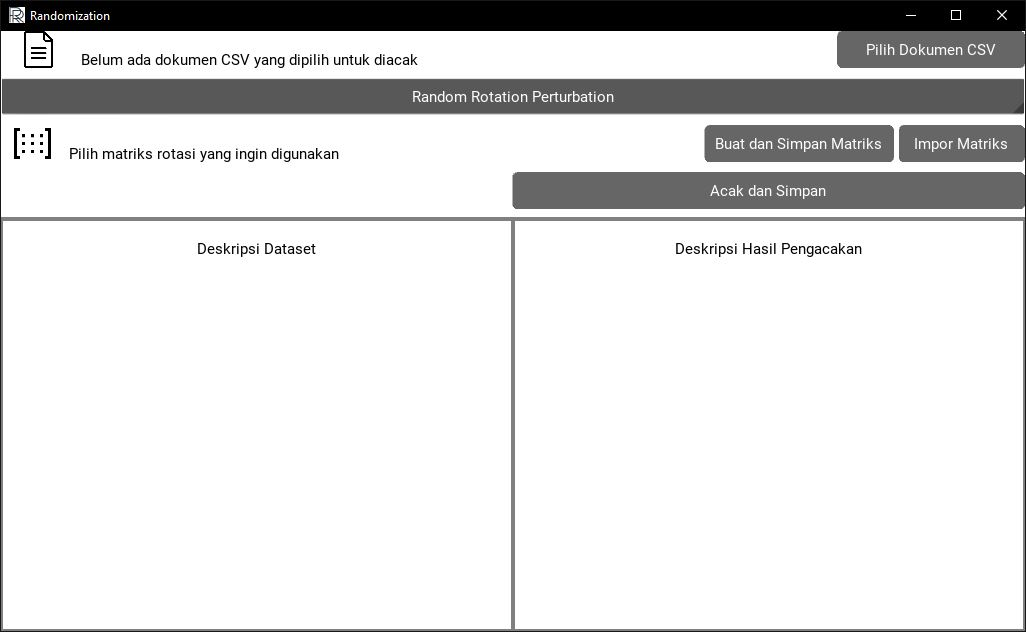
\includegraphics[scale=0.6]{antarmukautama}
	\caption{Tampilan perangkat lunak yang pertama ditampilkan saat perangkat lunak baru dibuka}
	\label{fig:antarmukautama}
\end{figure}

Antarmuka perangkat lunak mempunyai tiga buah bagian yang mempunyai fungsinya masing-masing. Ketiga bagian ini dapat dilihat pada Gambar~\ref{fig:antarmukautamabernomor} Pertama adalah bagian masukan dan pengaturan, terdapat pada bagian atas yang bernomor satu dan dikelilingi kotak merah. Kedua adalah bagian deskripsi \textit{dataset}, terdapat pada bagian bawah sebelah kiri yang bernomor dua dan dikelilingi kotak biru. Terakhir adalah bagian deskripsi hasil pengacakan, terdapat pada bagian bawah sebelah kanan yang bernomor tiga dan dikelilingi kotak hijau. Ketiga bagian ini akan dijelaskan secara rinci pada subbab-subbab berikutnya.

\begin{figure}
	\centering
	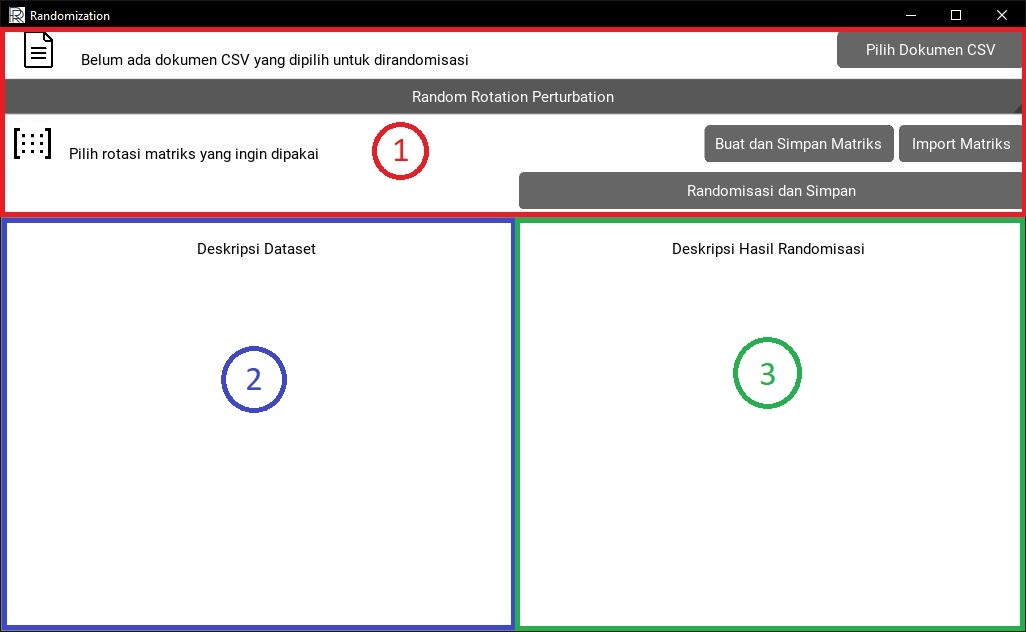
\includegraphics[scale=0.6]{antarmukautamabernomor}
	\caption{Bagian-bagian pada antarmuka perangkat lunak}
	\label{fig:antarmukautamabernomor}
\end{figure}

Perangkat lunak \textit{Randomization} mengimplementasikan dua buah teknik \textit{Randomization} yang berbeda yaitu \textit{Random Rotation Perturbation} dan \textit{Random Projection Perturbation}. Oleh karena itu, antarmuka perangkat lunak akan menyesuaikan dengan teknik yang dipilih oleh pengguna. Ketiga bagian antarmuka yang telah disebutkan tadi dengan otomatis akan berubah sesuai dengan teknik yang dipilih. Pada setiap subbab akan dijelaskan juga sekaligus perbedaan antarmuka teknik \textit{Randomization} satu dengan yang lainnya.

\subsection{Masukan dan Pengaturan}
\label{subsec:masukanpengaturan}

Bagian masukan dan pengaturan menyediakan berbagai interaksi untuk pengguna dapat mengatur masukan yang perlu diberikan kepada perangkat lunak dan menerapkan teknik \textit{Randomization} yang diinginkan. Ada beberapa fungsi inti pada bagian ini yaitu sebagai berikut.
\begin{itemize}
	\item Masukan \textit{dataset} berupa file \textit{comma-separated values} yang ingin diacak.
	\item Memilih teknik \textit{Randomization} yang ingin digunakan.
	\item Membuat baru dan memilih matriks rotasi atau proyeksi yang ingin digunakan.
	\item Masukan nilai variabel \textit{epsilon} dan nilai variabel \textit{k} untuk teknik \textit{Random Projection Perturbation}.
	\item Sebuah tombol untuk menerapkan teknik \textit{Randomization} dan menyimpan hasilnya.
\end{itemize}
Berikut akan dijelaskan secara rinci dengan gambar setiap fungsi tersebut yang dapat dilihat pada Gambar~\ref{fig:antarmukamasukanpengaturan} dan cara pemakaiannya yang benar secara berturut. 

\begin{figure}
	\centering
	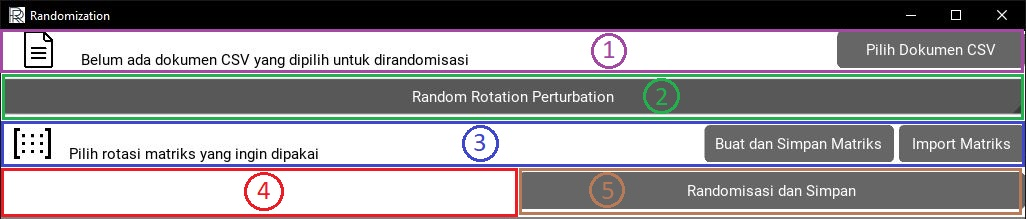
\includegraphics[scale=0.6]{antarmukamasukanpengaturan}
	\caption{Bagian antarmuka masukan dan pengaturan perangkat lunak}
	\label{fig:antarmukamasukanpengaturan}
\end{figure}

\subsubsection{Masukan \textit{Dataset}}
\label{subsubsec:masukandataset}

Pertama pengguna perlu memberikan masukan \textit{dataset} yang ingin diacak berupa dokumen berjenis \textit{comma-separated values}. Perangkat lunak menyediakan fitur tersebut yang dapat dilihat pada Gambar~\ref{fig:antarmukamasukanpengaturan} yang terdapat pada bagian yang dikelilingi kotak berwarna merah dan bernomor satu. Pengguna dapat menekan tombol \textquotedblleft Pilih Dokumen CSV\textquotedblright~yang terletak pada ujung sebelah kanan. Tombol ini bertujuan untuk memilih dokumen yang ingin diacak pada direktori pengguna. Ketika tombol ditekan, perangkat lunak akan membuka jendela baru untuk memilih dokumen yang dapat dilihat pada gambar~\ref{fig:pilihdokumen}.

\begin{figure}
	\centering
	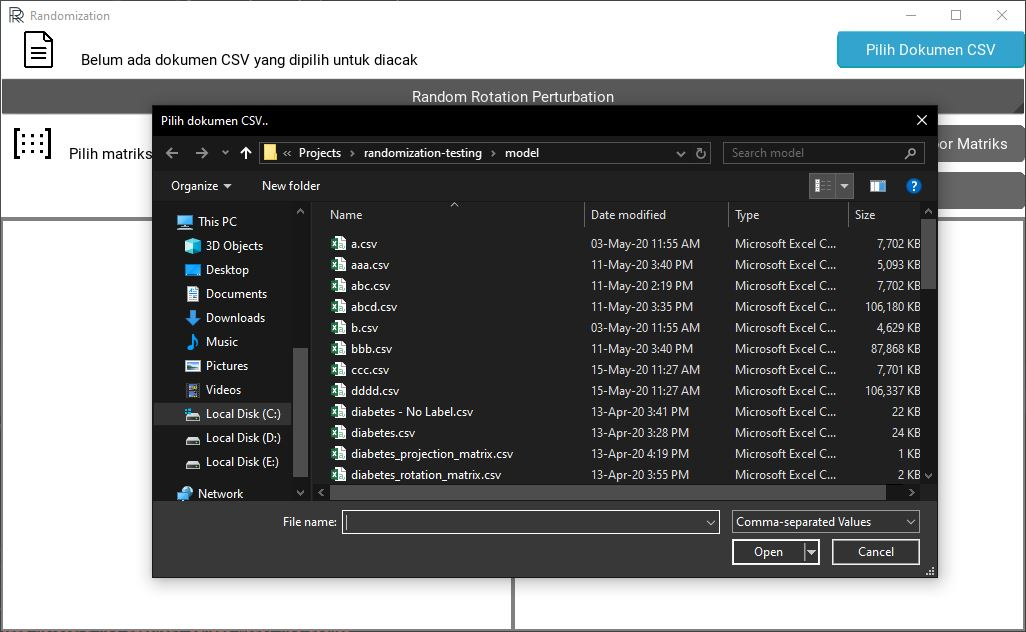
\includegraphics[scale=0.6]{pilihdokumen}
	\caption{Jendela untuk memilih \textit{dataset} yang berupa dokumen CSV}
	\label{fig:pilihdokumen}
\end{figure}

Setelah pengguna memilih \textit{dataset} yang diinginkan, perangkat lunak akan otomatis menuliskan lokasi dokumen yang dipilih berada. Perangkat lunak akan menampilkan lokasi dokumen tersebut pada bagian tengah sebelah kanan simbol dokumen dan sebelah kiri tombol \textquotedblleft Pilih Dokumen CSV\textquotedblright. Jika belum ada \textit{dataset} yang dipilih maka perangkat lunak akan menampilkan label yang berupa kalimat \textquotedblleft Belum ada dokumen CSV yang dipilih untuk diacak\textquotedblright~yang menunjukkan bahwa belum ada dokumen yang dipilih oleh pengguna. Jika pengguna memilih ulang dokumen, maka secara otomatis juga perangkat lunak akan memperbaharui lokasi dokumen sesuai dokumen yang dipilih pengguna.

Apabila dokumen yang dipilih berukuran besar, maka perangkat lunak akan memakan sedikit waktu yang lebih lama. Dalam rangka memberitahukan kepada pengguna bahwa perangkat lunak sedang melakukan proses pemilihan dokumen, perangkat lunak akan menampilkan sebuah \textit{popup} yang memberitahukan bahwa proses pemilihan sedang berjalan dan perangkat lunak tidak berhenti bekerja atau ada kesalahan sehingga pengguna tidak bingung apabila perangkat lunak memakan waktu yang lebih lama untuk memproses dokumen yang dipilih. Tampilan antarmuka \textit{popup} tersebut dapat dilihat pada Gambar~\ref{fig:loadingmemilihdokumen}. Setelah dokumen dipilih pengguna dan perangkat lunak berhasil memproses dokumen tersebut, perangkat lunak akan memperbaharui lokasi dokumen dan menampilkan beberapa informasi \textit{dataset} yang dipilih pada bagian deskripsi \textit{dataset} yang akan dijelaskan pada subbab berikutnya. Tampilan antarmuka setelah pengguna memilih dokumen dapat dilihat pada Gambar~\ref{fig:dokumendipilih}

\begin{figure}
	\centering
	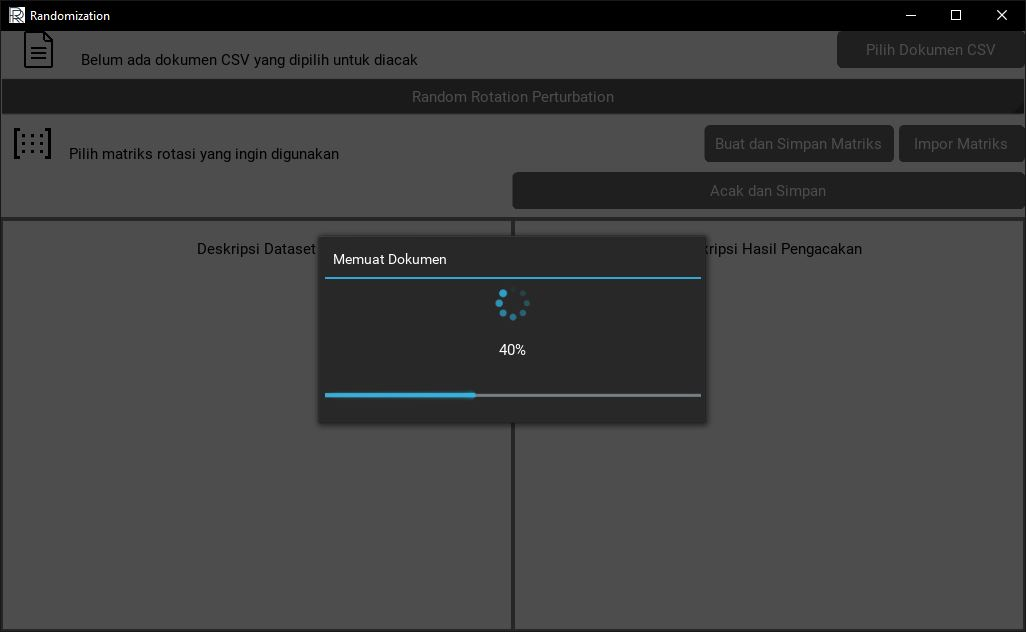
\includegraphics[scale=0.6]{loadingmemilihdokumen}
	\caption{Tampilan \textit{popup} yang ditampilkan saat proses berlangsung}
	\label{fig:loadingmemilihdokumen}
\end{figure}

\begin{figure}
	\centering
	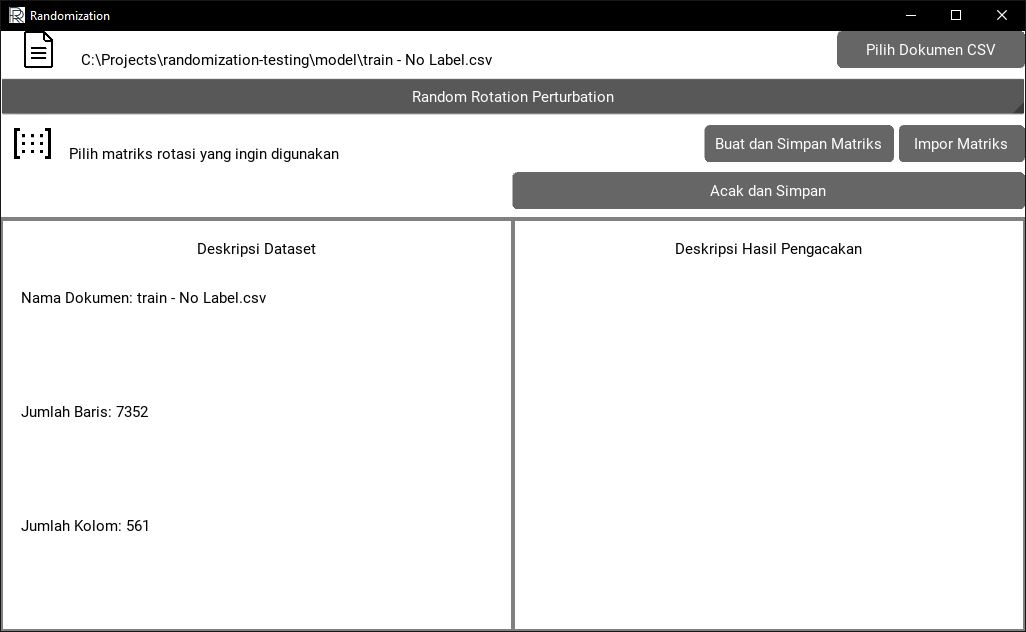
\includegraphics[scale=0.6]{dokumendipilih}
	\caption{Tampilan antarmuka setelah sebuah dokumen dipilih}
	\label{fig:dokumendipilih}
\end{figure}

Selain itu setelah pengguna memilih dokumen CSV, perangkat lunak akan membaca dokumen tersebut dan memproses isi dari dokumen tersebut menjadi \textit{dataset} yang berupa matriks. Proses ini dilakukan sekali saja tepat setelah pengguna memilih dokumen dengan menekan tombol \textquotedblleft Pilih Dokumen CSV\textquotedblright. Oleh karena itu, apabila sebuah dokumen CSV diubah isinya setelah dokumen tersebut dipilih oleh pengguna maka perangkat lunak tetap akan menggunakan isi dari dokumen tersebut yang belum diubah. Pengguna harus berhati-hati apabila isi dokumen diubah maka pengguna juga harus memilih kembali dokumen yang sama tersebut walaupun perangkat lunak sudah menunjukkan lokasi dokumen yang digunakan adalah dokumen yang pengguna inginkan.

\subsubsection{Pemilihan teknik \textit{Randomization}}
\label{subsubsec:pilihteknik}

Setelah pengguna memilih \textit{dataset} yang ingin diacak, pengguna juga harus memilih teknik \textit{Randomization} apa yang ingin diterapkan terhadap \textit{dataset} yang sudah dipilih. Pada awal perangkat lunak dibuka, secara otomatis teknik \textit{Random Rotation Perturbation} yang dipilih. Apabila pengguna ingin mengganti teknik yang ingin diterapkan pada \textit{dataset}, pengguna dapat menekan tombol \textit{dropdown} yang bertuliskan nama teknik \textit{Randomization}. Tombol ini dapat dilihat pada Gambar~\ref{fig:antarmukamasukanpengaturan} yang dikelilingi kotak berwarna hijau dan bernomor dua.

Apabila pengguna menekan tombol ini maka perangkat lunak akan menampilkan \textit{dropdown} yang mempunyai dua buah opsi teknik \textit{Randomization} yaitu \textquotedblleft Random Rotation Perturbation\textquotedblright~dan \textquotedblleft Random Projection Perturbation\textquotedblright. Antarmuka tersebut dapat dilihat pada Gambar~\ref{fig:opsipilihteknik} yang dikelilingi oleh kotak merah. Pemilihan teknik ini juga akan memicu beberapa perubahan pada tampilan antarmuka perangkat lunak menyesuaikan dengan teknik yang dipilih. Beberapa perubahan pada perangkat lunak tersebut melingkupi bagian pembuatan dan pemilihan matriks, parameter teknik \textit{Randomization}, dan bagian pengacakan dan simpan yang akan dijelaskan setiap perubahan tersebut pada subbab berikutnya.

\begin{figure}
	\centering
	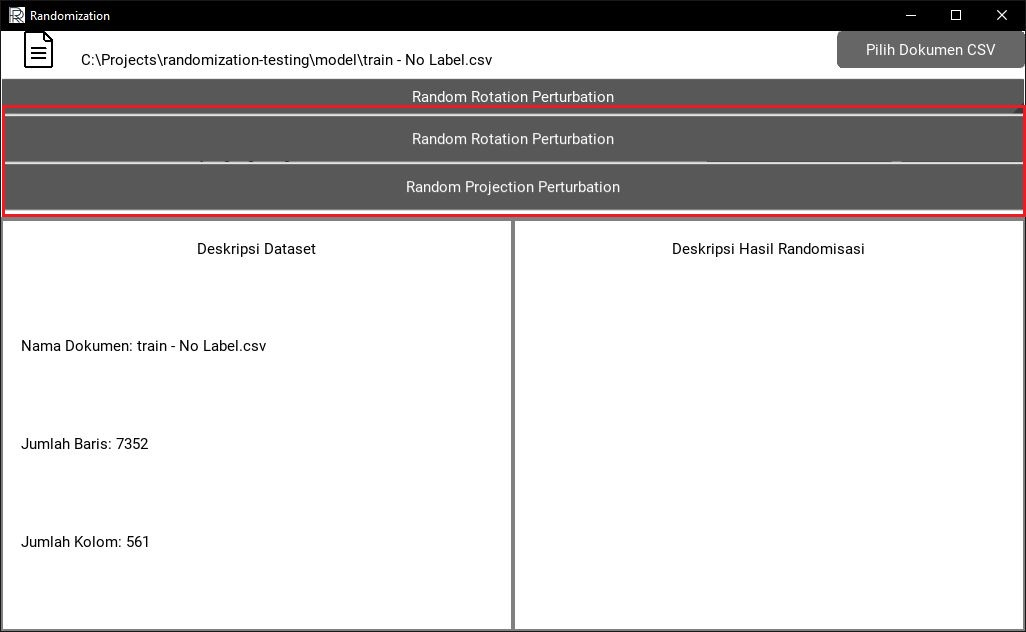
\includegraphics[scale=0.6]{opsipilihteknik}
	\caption{Tampilan antarmuka saat pengguna memilih teknik}
	\label{fig:opsipilihteknik}
\end{figure}

\subsubsection{Pembuatan dan Pemilihan Matriks}
\label{subsubsec:pilihmatriks}

Setelah pengguna memilih teknik yang ingin diterapkan, pengguna harus memilih matriks yang diinginkan atau membuat baru. Matriks yang dimaksudkan adalah matriks rotasi atau matriks proyeksi sesuai teknik \textit{Randomization} yang dipilih. Apabila teknik \textit{Random Rotation Perturbation} yang dipilih maka perangkat lunak akan mengubah fungsi pembuatan dan pemilihan matriks ini menjadi matriks rotasi. Apabila teknik \textit{Random Projection Perturbation} yang dipilih maka perangkat lunak akan mengubah fungsi pembuatan dan pemilihan matriks ini menjadi matriks proyeksi. Perubahan ini dapat terlihat pada label yang berada di sebelah kanan simbol matriks apabila belum memilih atau membuat matriks maka label tersebut akan menampilkan kalimat \textquotedblleft Pilih matriks rotasi yang ingin digunakan\textquotedblright~atau \textquotedblleft Pilih matriks proyeksi yang ingin digunakan\textquotedblright. Bagian ini dapat dilihat pada Gambar~\ref{fig:antarmukamasukanpengaturan} yang dikelilingi oleh kotak berwarna hijau dan bernomor dua.

Ada dua buah tombol pada bagian ini yaitu \textquotedblleft Buat dan Simpan Matriks\textquotedblright~dan \textquotedblleft Import Matriks\textquotedblright. Tombol \textquotedblleft Buat dan Simpan Matriks\textquotedblright~mempunyai fungsi untuk membuat matriks rotasi atau proyeksi baru sesuai teknik \textit{Randomization} yang dipilih dan menyimpan matriks tersebut pada sebuah dokumen CSV baru yang dibuat oleh perangkat lunak pada direktori tertentu yang akan dipilih oleh pengguna. Pada saat perangkat lunak sedang memproses matriks tersebut, perangkat lunak akan menampilkan \textit{popup} memuat yang dapat dilihat pada Gambar~\ref{fig:buatsimpanmatriks}. \textit{Popup} ini juga akan tampil saat proses impor matriks dilakukan. Hasil matriks yang dibuat oleh perangkat lunak dapat digunakan kembali untuk lain kali sehingga rotasi atau proyeksi yang diterapkan akan sama dengan yang sebelumnya. 

Pengguna dapat melakukan impor matriks dengan cara menekan tombol \textquotedblleft Import Matriks\textquotedblright~untuk memilih matriks rotasi atau proyeksi yang diinginkan untuk diterapkan pada \textit{dataset}. Matriks yang dipilih harus sesuai dengan \textit{dataset} yang ingin diacak, misalnya apabila matriks rotasi yang dipilih memiliki dimensi yang berbeda dengan \textit{dataset} maka perangkat lunak akan melarang impor matriks dilakukan karena pengacakan tidak dapat dilakukan. Perangkat lunak akan menampilkan \textit{popup} peringatan untuk pengguna yang dapat dilihat pada Gambar~\ref{fig:matrikstidaksesuai}. Apabila pengguna memilih teknik \textit{Random Projection Perturbation} dan pengguna mengimpor matriks proyeksi maka parameter variabel \textit{k} akan terisi secara otomatis sesuai dengan matriks proyeksi yang diimpor.

\begin{figure}
	\centering
	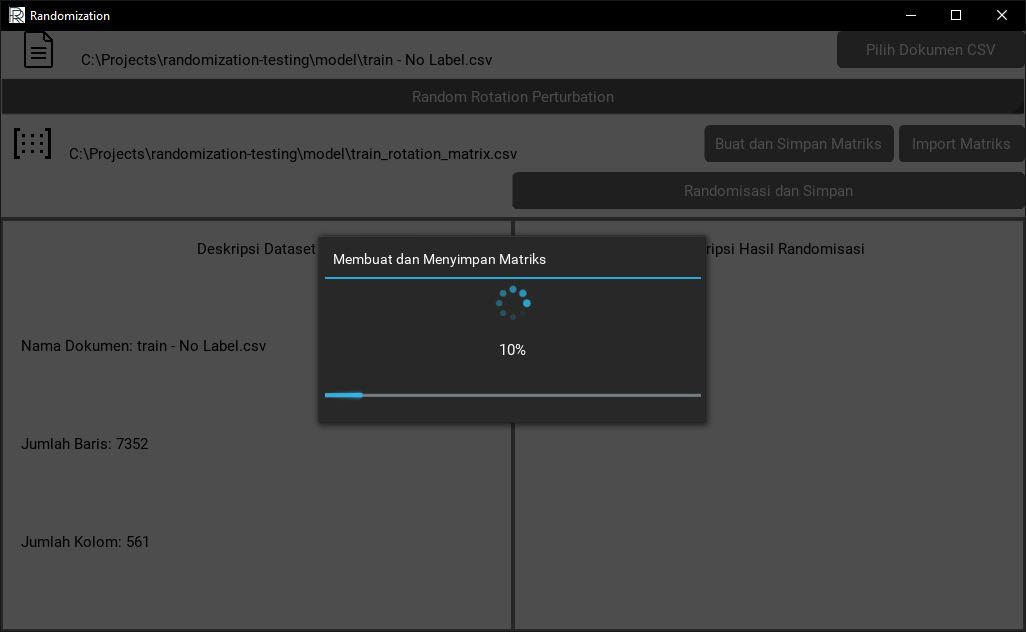
\includegraphics[scale=0.6]{buatsimpanmatriks}
	\caption{Tampilan antarmuka saat perangkat lunak membuat dan menyimpan matriks}
	\label{fig:buatsimpanmatriks}
\end{figure}

\begin{figure}
	\centering
	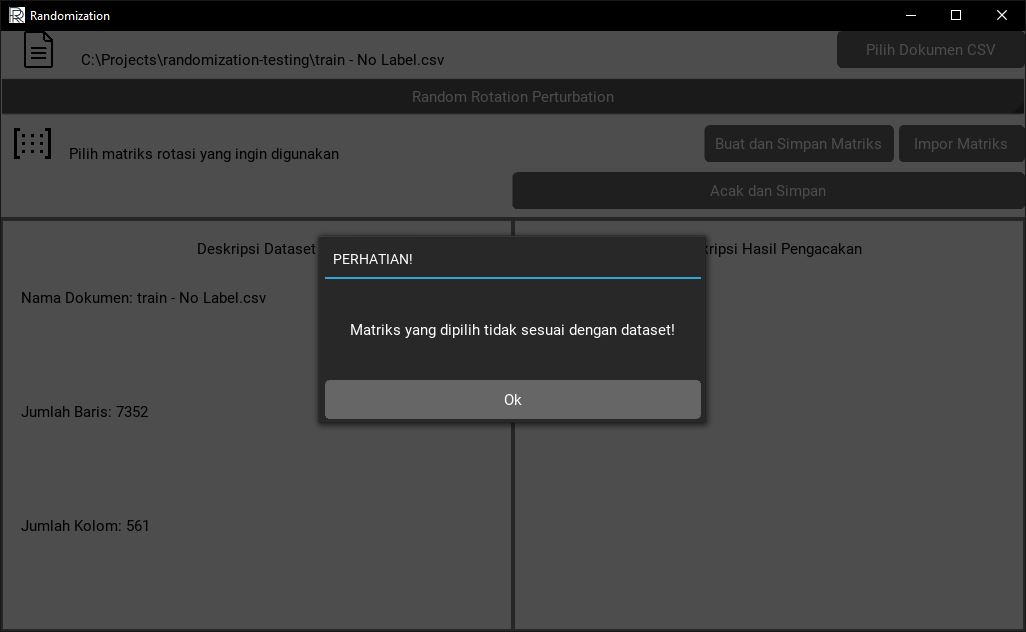
\includegraphics[scale=0.6]{matrikstidaksesuai}
	\caption{Tampilan \textit{popup} yang ditampilkan apabila matriks yang ingin diimpor tidak sesuai dengan \textit{dataset}}
	\label{fig:matrikstidaksesuai}
\end{figure}

Apabila pengguna belum memilih \textit{dataset} yang ingin diacak, pengguna tidak dapat membuat maupun impor matriks terlebih dahulu. Hal ini dikarenakan perlu ada proses pengecekan terlebih dahulu yang dilakukan perangkat lunak untuk memastikan \textit{dataset} yang ingin diacak sudah sesuai persyaratan dan sesuai dengan matriks yang akan dipilih. Perangkat lunak akan melarang pengguna membuat maupun impor matriks dengan menampilkan sebuah \textit{popup} peringatan yang dapat dilihat pada Gambar~\ref{fig:larangmatriks}. Pada teknik \textit{Random Projection Perturbation}, pengguna baru bisa membuat matriks proyeksi apabila sudah memenuhi persyaratan yang diminta yaitu mengisi parameter teknik tersebut yang mana adalah variabel \textit{epsilon} dan variabel \textit{k}.

\begin{figure}
	\centering
	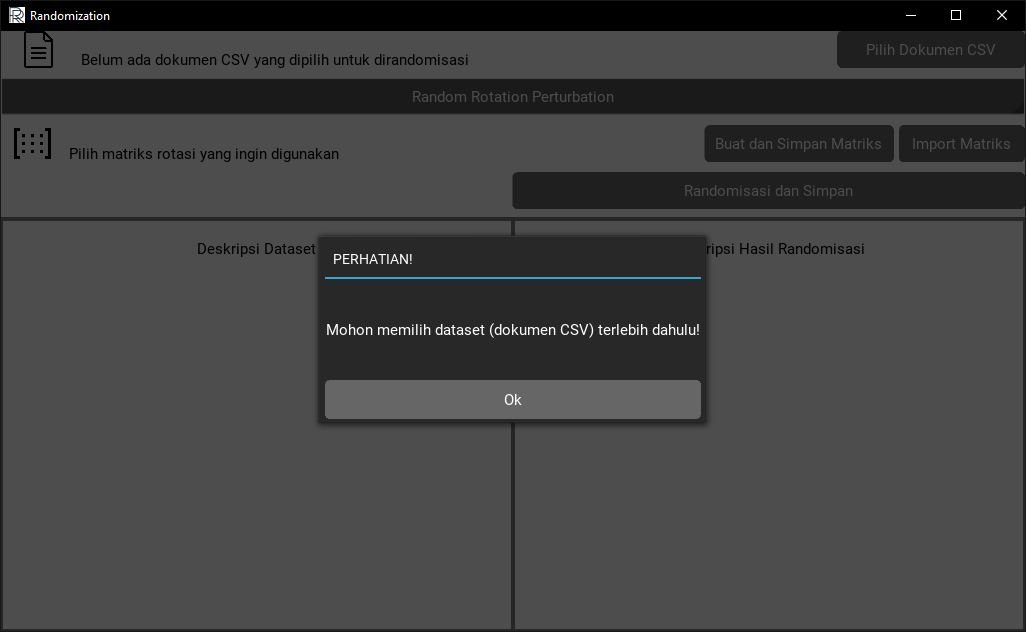
\includegraphics[scale=0.6]{larangmatriks}
	\caption{Tampilan \textit{popup} yang ditampilkan apabila pengguna belum memilih \textit{dataset} yang ingin diacak}
	\label{fig:larangmatriks}
\end{figure}

\subsubsection{Parameter teknik \textit{Randomization}}
\label{subsubsec:parameterteknik}

Perangkat lunak hanya meminta kepada pengguna parameter untuk teknik \textit{Random Projection Perturbation} saja apabila pengguna memilih teknik tersebut. Pada teknik \textit{Random Rotation Perturbation} tidak ada parameter yang perlu pengguna berikan. Ada dua buah parameter yang perlu pengguna berikan yaitu variabel \textit{epsilon} dan variabel \textit{k}. Pengguna dapat memasukkan nilai kedua variabel tersebut dengan menekan kolom variabel tersebut masing-masing. Kedua buah parameter tersebut dapat dilihat antarmukanya pada Gambar~\ref{fig:parameterprojection}

\begin{figure}
	\centering
	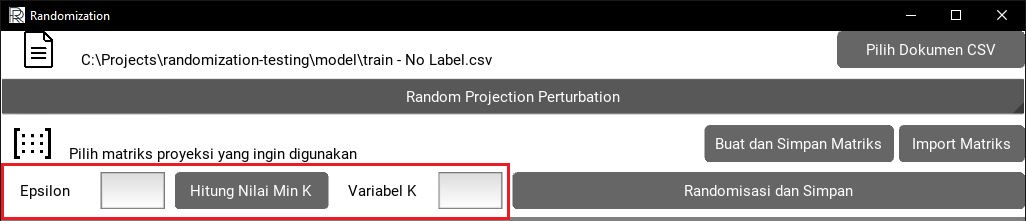
\includegraphics[scale=0.6]{parameterprojection}
	\caption{Tampilan antarmuka parameter teknik \textit{Randomization} \textit{Random Projection Perturbation}}
	\label{fig:parameterprojection}
\end{figure}

Seperti yang disinggung pada subbab sebelumnya antarmuka perangkat lunak akan menyesuaikan secara otomatis sesuai teknik yang dipilih pengguna. Pada bagian parameter teknik \textit{Randomization}, perangkat lunak akan menyembunyikan antarmuka parameter \textit{Random Projection Perturbation} apabila pengguna memilih teknik \textit{Random Rotation Perturbation}. Antarmuka tersebut dapat dilihat pada Gambar~\ref{fig:antarmukamasukanpengaturan} yang dikelilingi oleh kotak berwarna merah dan bernomor empat, dapat dilihat tidak ada parameter apapun yang tampil apabila teknik \textit{Random Rotation Perturbation} yang dipilih.

Selain dua buah parameter, pada bagian ini juga ada sebuah tombol yaitu \textquotedblleft Hitung Nilai Min K\textquotedblright~yang memiliki fungsi untuk menghitung nilai minimal variabel \textit{k} yang pengguna berikan. Pada teknik \textit{Random Projection Perturbation}, ada beberapa persyaratan yang harus dipenuhi oleh pengguna dan salah satunya adalah variabel \textit{k} yang diberikan harus melebihi sebuah nilai minimal yang dihitung berdasarkan ukuran \textit{dataset} dan nilai variabel \textit{epsilon}. Oleh karena itu, sebelum tombol ini dapat berfungsi, pengguna harus memilih terlebih dahulu \textit{dataset} yang ingin diacak dan memberikan masukan nilai variabel \textit{epsilon} yang sesuai dengan persyaratan variabel \textit{epsilon} yaitu nilainya lebih besar dari 0 dan kurang dari 1. Apabila pengguna belum memenuhi kedua persyaratan tersebut, tombol tidak akan berfungsi dan perangkat lunak akan menampilkan \textit{popup} peringatan yang dapat dilihat pada Gambar~\ref{fig:popuphitungk}. Nilai minimal variabel \textit{k} akan ditampilkan pada bagian antarmuka deskripsi \textit{dataset} yang akan dijelaskan pada subbab berikutnya.

\begin{figure}
	\centering
	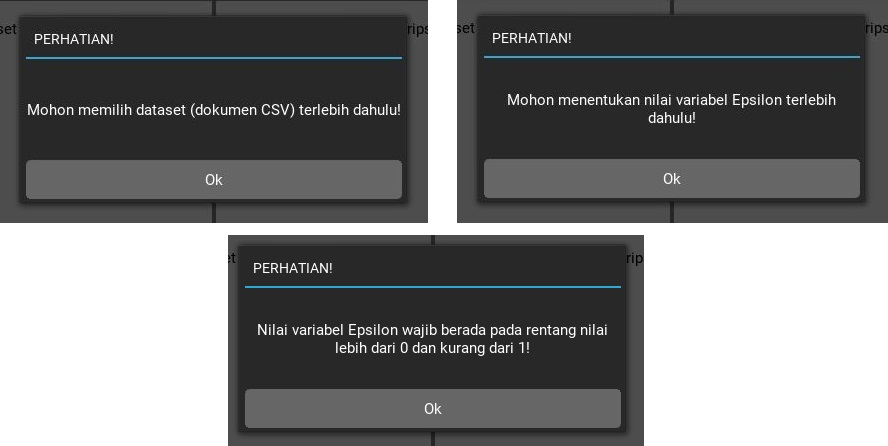
\includegraphics[scale=0.6]{popuphitungk}
	\caption{Tampilan \textit{popup} peringatan tombol \textquotedblleft Hitung Nilai Min K\textquotedblleft }
	\label{fig:popuphitungk}
\end{figure}

Perangkat lunak juga akan memberikan peringatan apabila nilai minimal \textit{k} melebihi dimensi dari \textit{dataset} yang ingin diacak karena salah satu persyaratan dari teknik \textit{Random Projection Perturbation} adalah nilai variabel \textit{k} harus lebih kecil daripada jumlah dimensi pada \textit{dataset} yang ingin diacak. Apabila pengguna melakukan impor matriks maka variabel \textit{k} akan terisi secara otomatis dan pengguna harus menyesuaikan nilai variabel \textit{epsilon} dengan variabel \textit{k} yang tidak boleh diubah oleh pengguna. 

\subsubsection{Pengacakan dan Simpan}
\label{subsubsec:randomisasisimpan}

Setelah pengguna memberikan masukan yang sesuai dan mengatur pengaturan yang diinginkan maka pengguna telah dapat melakukan pengacakan dengan menekan tombol \textquotedblleft Acak dan Simpan\textquotedblright. Tombol ini akan menerapkan teknik \textit{Randomization} yang dipilih oleh pengguna terhadap \textit{dataset} yang ingin diacak menggunakan matriks yang telah dibuat atau dipilih oleh pengguna dan parameter-parameter yang pengguna berikan. Tampilan antarmuka saat proses pengacakan dilakukan perangkat lunak dapat dilihat pada Gambar~\ref{fig:loadingrandomisasi}.

\begin{figure}
	\centering
	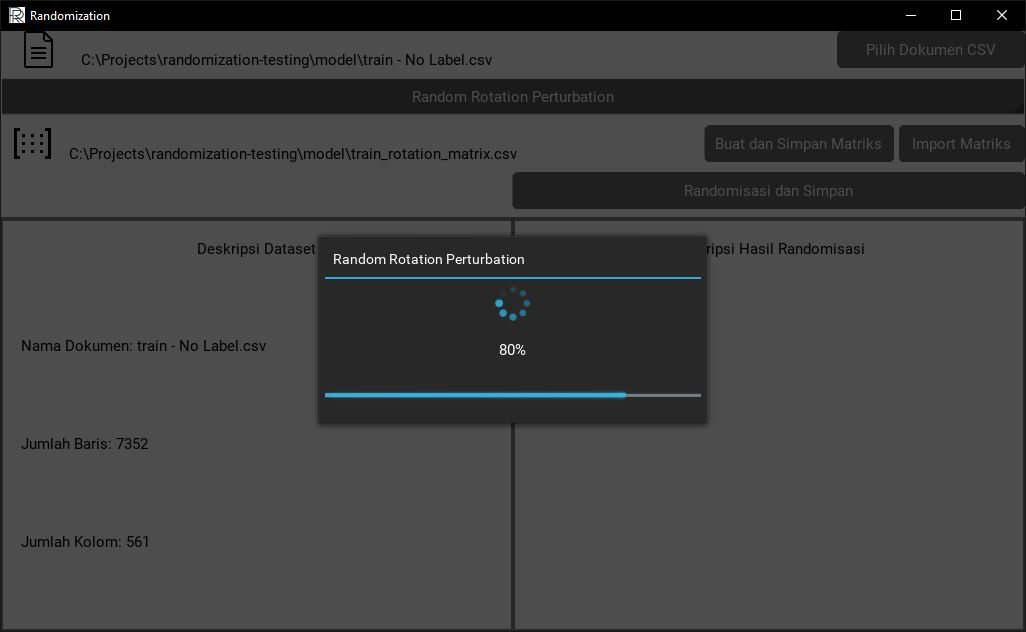
\includegraphics[scale=0.6]{loadingrandomisasi}
	\caption{Tampilan saat perangkat lunak sedang melakukan proses pengacakan}
	\label{fig:loadingrandomisasi}
\end{figure}

Setelah perangkat lunak berhasil melakukan pengacakan, perangkat lunak akan meminta pengguna untuk memilih direktori tempat penyimpanan dan nama dokumen hasil pengacakan. Perangkat lunak akan menyimpan hasil pengacakan dalam bentuk dokumen berjenis \textit{comma-separated values}. Jendela baru untuk memilih direktori penyimpanan akan ditampilkan perangkat lunak, apabila pengguna membatalkan atau dengan kata lain menutup jendela tersebut tanpa memilih direktori penyimpanan maka perangkat lunak tidak akan melanjutkan proses pengacakan dan dianggap gagal. Tampilan antarmuka \textit{popup} yang akan tampil setelah perangkat lunak berhasil melakukan proses pengacakan dan menyimpan hasilnya pada direktori yang pengguna pilih dapat dilihat pada Gambar~\ref{fig:popupberhasilrandomisasi}. Perangkat lunak juga akan menampilkan berbagai informasi hasil pengacakan pada bagian antarmuka deskripsi hasil pengacakan yang akan dijelaskan pada subbab berikutnya.

\begin{figure}
	\centering
	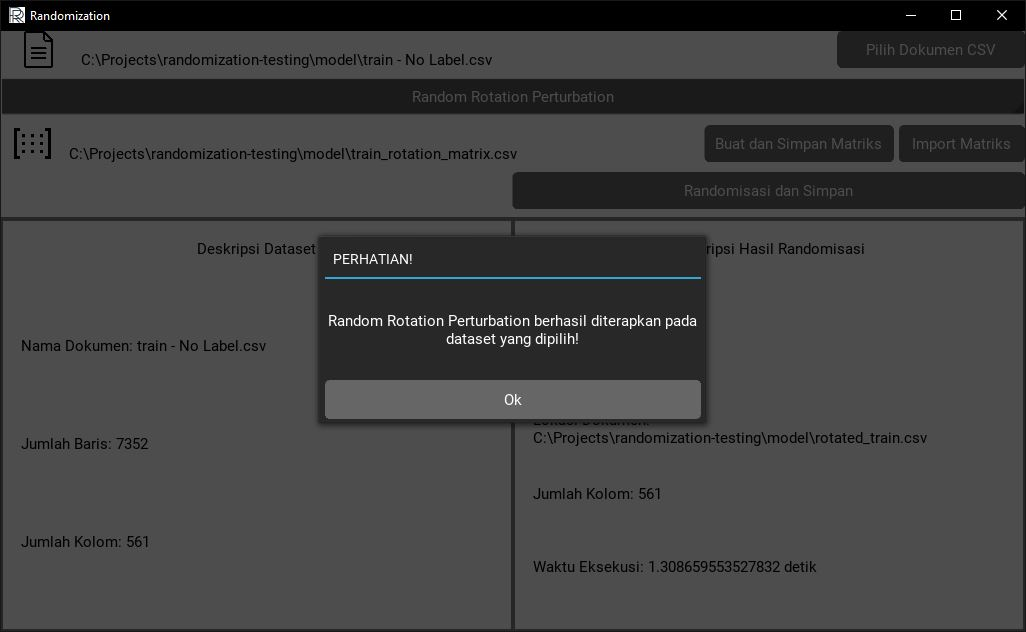
\includegraphics[scale=0.6]{popupberhasilrandomisasi}
	\caption{Tampilan \textit{popup} untuk memberitahukan pengguna bahwa pengacakan berhasil dilakukan}
	\label{fig:popupberhasilrandomisasi}
\end{figure}

Ada beberapa persyaratan yang harus dipenuhi oleh pengguna sebelum melakukan pengacakan yaitu sebagai berikut.
\begin{itemize}
	\item Memilih \textit{dataset} yang ingin diacak.
	\item Memilih teknik \textit{Randomization} yang diinginkan.
	\item Membuat atau memilih matriks rotasi atau proyeksi.
	\item Memberikan masukan nilai variabel \textit{epsilon} dan nilai variabel \textit{k}.
\end{itemize}
Persyaratan terakhir hanya berlaku apabila pengguna memilih teknik \textit{Random Projection Perturbation}. Apabila ada persyaratan yang tidak dipenuhi oleh pengguna maka perangkat lunak akan menampilkan \textit{popup} untuk memberikan peringatan kepada pengguna dan perangkat lunak tidak akan melanjutkan proses pengacakan. Perangkat lunak akan menampilkan \textit{popup} peringatan terhadap pelanggaran masing-masing persyaratan tersebut, salah satu contoh tampilan antarmuka \textit{popup} tersebut dapat dilihat pada Gambar~\ref{fig:popupdataset}.

\begin{figure}
	\centering
	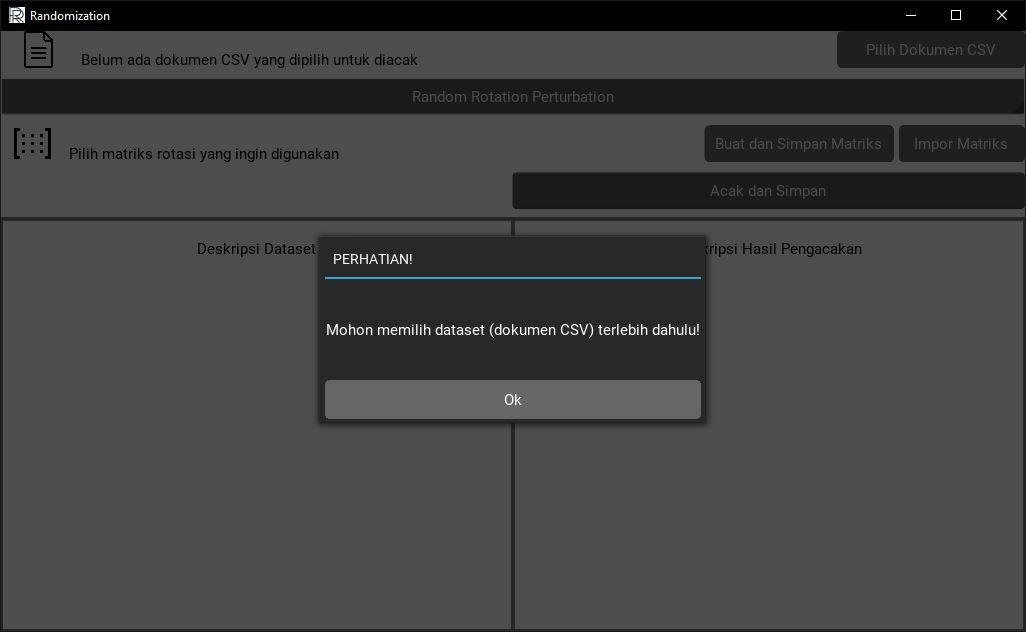
\includegraphics[scale=0.6]{popupdataset}
	\caption{Tampilan \textit{popup} peringatan apabila pengguna belum memilih \textit{dataset} yang diinginkan untuk diacak}
	\label{fig:popupdataset}
\end{figure}

\subsection{Deskripsi \textit{Dataset}}
\label{subsec:deskripsidataset}

Pengguna dapat melihat berbagai informasi dokumen \textit{comma-separated values} yang dipilih sebagai \textit{dataset} yang ingin diacak pada bagian antarmuka deskripsi \textit{dataset} yaitu sebagai berikut. 
\begin{itemize}
	\item Nama dokumen
	\item Jumlah baris \textit{dataset}
	\item Jumlah kolom \textit{dataset}
	\item Nilai minimal variabel \textit{k}
\end{itemize}
Seperti yang disinggung pada subbab sebelumnya, pada awalnya nilai minimal variabel \textit{k} belum diketahui karena belum dihitung. Pengguna harus mengisi variabel \textit{epsilon} dan menekan tombol \textquotedblleft Hitung Nilai Min K\textquotedblright~agar perangkat lunak menghitung nilai minimal variabel \textit{k} dan dapat menampilkannya pada deskripsi \textit{dataset}. Nilai minimal variabel \textit{k} hanya ditampilkan apabila pengguna memilih teknik \textit{Random Projection Perturbation}.

Bagian antarmuka deskripsi \textit{dataset} ini akan selalu secara otomatis diperbaharui setiap pengguna memilih \textit{dataset} baru. Tampilan antarmuka bagian deskripsi \textit{dataset} dapat dilihat pada Gambar~\ref{fig:antarmukautamabernomor} yang dikelilingi oleh kotak berwarna biru dan bernomor dua. Apabila pengguna telah memilih \textit{dataset} yang diinginkan untuk diacak maka perangkat lunak secara otomatis akan memperbaharui tampilan antarmuka deskripsi \textit{dataset} yang dapat dilihat pada Gambar~\ref{fig:antarmukadeskripsidataset}

\begin{figure}
	\centering
	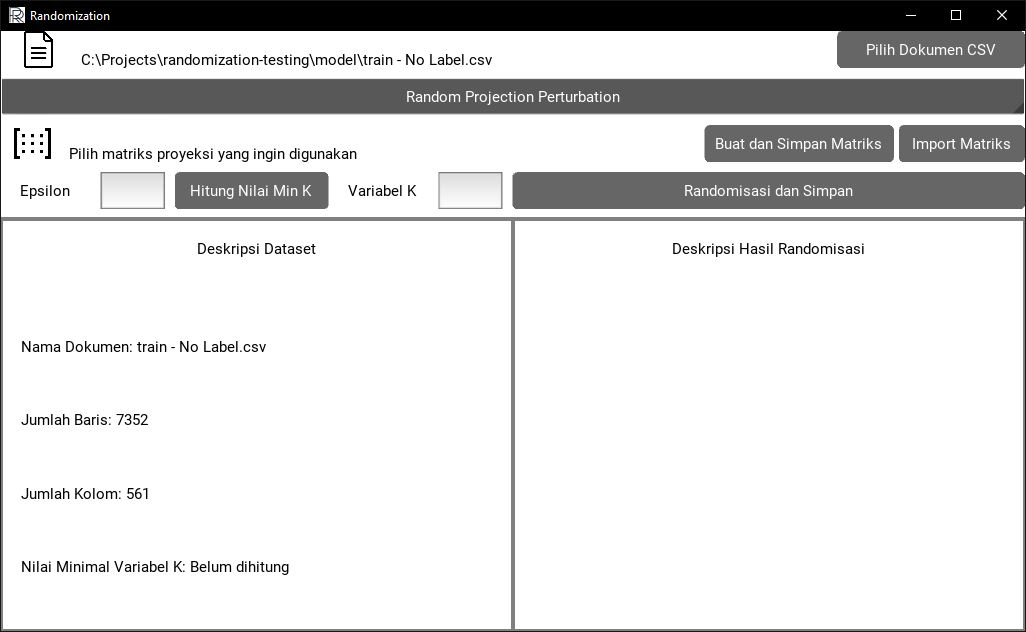
\includegraphics[scale=0.6]{antarmukadeskripsidataset}
	\caption{Tampilan antarmuka deskripsi \textit{dataset} setelah pengguna memilih \textit{dataset} yang ingin diacak}
	\label{fig:antarmukadeskripsidataset}
\end{figure}

\subsection{Deskripsi Hasil Pengacakan}
\label{subsec:deskripsihasil}

Perangkat lunak akan menampilkan isi dari deskripsi hasil pengacakan setelah pengguna menekan tombol \textquotedblleft Acak dan Simpan\textquotedblright~dan perangkat lunak melakukan proses pengacakan. Bagian deskripsi hasil pengacakan ini akan menampilkan informasi sebagai berikut. 
\begin{itemize}
	\item Status
	\item Lokasi dokumen
	\item Lokasi dokumen matriks yang dipakai
	\item Jumlah kolom
	\item Waktu eksekusi
	\item Nilai variabel \textit{epsilon} yang digunakan
	\item Nilai variabel \textit{k} yang digunakan
\end{itemize}
Nilai variabel \textit{epsilon} dan nilai variabel \textit{k} hanya ditampilkan apabila pengguna memilih teknik \textit{Randomization} \textit{Random Projection Perturbation}.

Bagian antarmuka deskripsi \textit{dataset} ini akan selalu secara otomatis diperbaharui setiap pengguna memilih \textit{dataset} baru. Tampilan antarmuka bagian deskripsi \textit{dataset} dapat dilihat pada Gambar~\ref{fig:antarmukautamabernomor} yang dikelilingi oleh kotak berwarna biru dan bernomor dua. Apabila pengguna telah memilih \textit{dataset} yang diinginkan untuk diacak maka perangkat lunak secara otomatis akan memperbaharui tampilan antarmuka deskripsi \textit{dataset} yang dapat dilihat pada Gambar~\ref{fig:antarmukahasilrandomisasi}

\begin{figure}
	\centering
	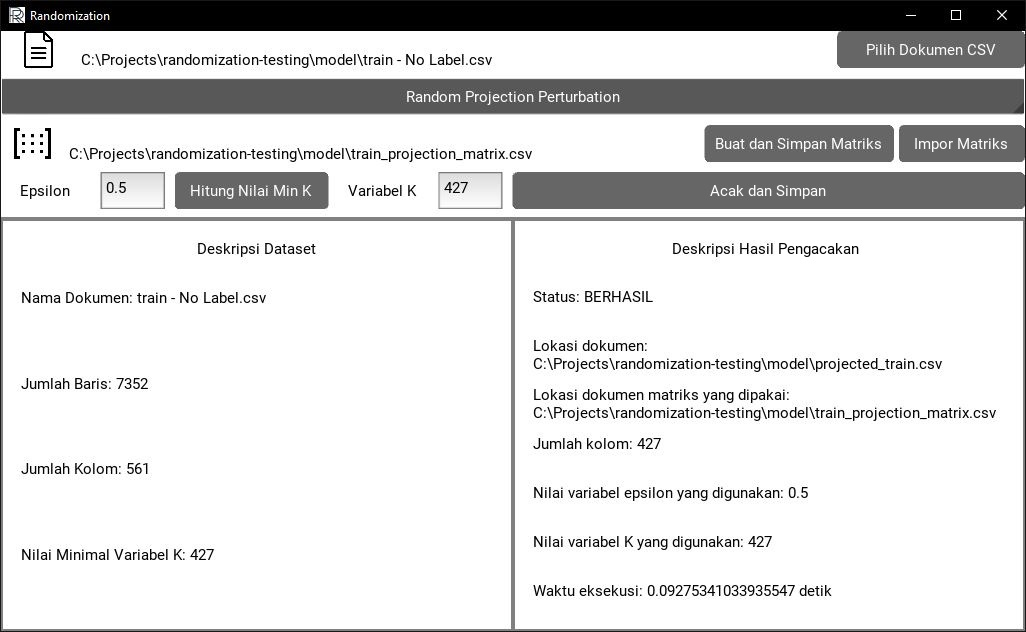
\includegraphics[scale=0.6]{antarmukahasilrandomisasi}
	\caption{Tampilan antarmuka deskripsi hasil pengacakan setelah perangkat berhasil melakukan pengacakan}
	\label{fig:antarmukahasilrandomisasi}
\end{figure}

\section{Pengujian Fungsional}
\label{sec:pengujianfungsional}

Pengujian fungsional bertujuan untuk memastikan perangkat lunak \textit{Randomization} dapat menerapkan kedua teknik \textit{Randomization} yaitu \textit{Random Rotation Perturbation} dan \textit{Random Projection Perturbation} dengan baik terhadap \textit{dataset} yang memenuhi syarat. Proses pengujian akan dilakukan dengan cara menerapkan kedua teknik tersebut dari awal memasukkan \textit{dataset} sampai menghasilkan \textit{dataset} yang telah diacak. Berikut pengujian pada setiap teknik \textit{Randomization} dengan menerapkan teknik penambangan data. Berikut pengujian pada setiap teknik \textit{Randomization} dengan menerapkan teknik penambangan data.

\subsection{Teknik \textit{Random Rotation Perturbation}}
\label{subsec:rrp-fungsional}

Pengujian teknik \textit{Random Rotation Perturbation} akan menggunakan \textit{dataset} \textit{mall\_customers}\footnote{https://www.kaggle.com/vjchoudhary7/customer-segmentation-tutorial-in-python} yang berisi informasi pribadi pelanggan sebuah mall. \textit{Dataset} ini memiliki 4 buah fitur yaitu jenis kelamin, umur, penghasilan, dan skor pengeluaran. Empat buah fitur tersebut akan diacak dan diharapkan hasilnya akan mengacak \textit{dataset} sehingga nilai tiap fitur tersebut berbeda dari aslinya. Selain itu, matriks rotasi harus dapat disimpan dan digunakan kembali untuk lain kali. \textit{Dataset} yang telah diacak juga diharapkan masih dapat diterapkan teknik penambangan data dengan hasil yang kualitasnya sama dengan \textit{dataset} asli, pengujian untuk hal ini akan dilakukan pada bagian berikutnya yaitu pada pengujian eksperimental.

Pada teknik \textit{Random Rotation Perturbation} untuk merotasikan sebuah \textit{dataset} diperlukan sebuah matriks rotasi dan translasi acak. Perangkat lunak diharapkan dapat membuat kedua matriks tersebut dan menyimpannya ke dalam sebuah dokumen \textit{comma-separated values}. Beberapa kolom pada \textit{dataset} \textit{mall\_customers} harus dihilangkan terlebih dahulu agar hanya fitur (bersifat numerik) pada \textit{dataset} tersebut saja yang teracak. \textit{Dataset} \textit{mall\_customers} mempunyai 3 buah fitur yang akan diacak, oleh karena itu matriks rotasi dan translasi acak yang dibuat perangkat lunak seharusnya berukuran \(3\times3\) kecuali matriks translasi yang akan berukuran \(4\times4\) karena matriks translasi mempunyai kolom terakhir tambahan yang dibutuhkan untuk melakukan tranformasi translasi. 

Pada pengujian yang dilakukan, perangkat lunak berhasil membuat kedua matriks acak tersebut dengan ukuran yang benar dan menyimpannya pada satu dokumen \textit{comma-separated values} yang isinya dapat dilihat pada Gambar~\ref{fig:mall_rotation_matrix}. Matriks rotasi dan translasi ini akan digunakan untuk menerapkan teknik \textit{Random Rotation Perturbation} terhadap \textit{dataset} \textit{mall\_customers}. Perangkat lunak juga berhasil menggunakan ulang kedua matriks yang telah disimpan tersebut untuk menerapkan teknik \textit{Random Rotation Perturbation} terhadap \textit{dataset} \textit{mall\_customers} dan hasilnya sama persis seperti hasil yang pertama kali. Kedua matriks tersebut juga dapat digunakan untuk data \textit{mall\_customers} yang lain dengan syarat masih memiliki jumlah fitur yang sama.

\begin{figure}
	\centering
	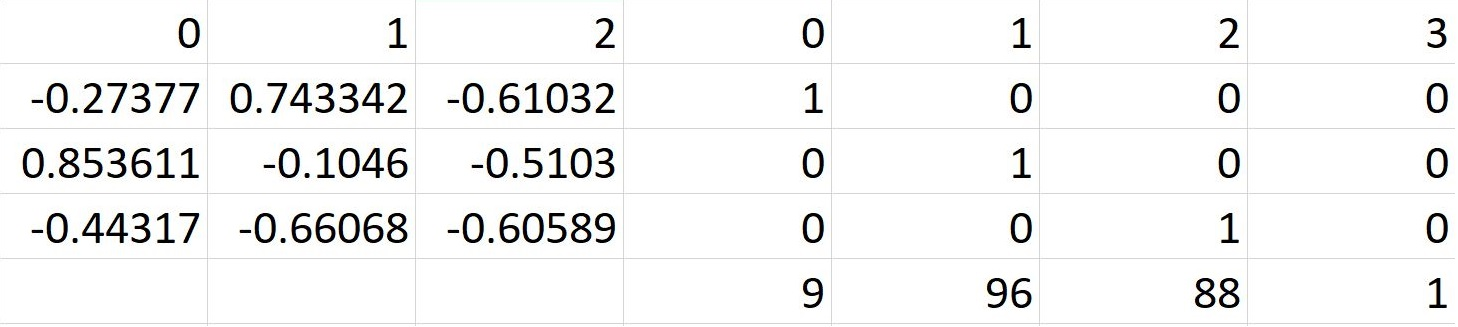
\includegraphics[scale=0.35]{mall_rotation_matrix}
	\caption{Matriks rotasi dan translasi acak yang dibuat perangkat lunak dan disimpan pada satu dokumen  \textit{comma-separated values}}
	\label{fig:mall_rotation_matrix}
\end{figure}

Berikut akan ditampilkan 20 baris pertama \textit{dataset} asli dan \textit{dataset} yang telah diacak masing-masing pada Gambar~\ref{fig:mall_customers_asli} dan Gambar~\ref{fig:rotated_mall_customers}. Dapat dilihat pada gambar tersebut, \textit{dataset} setelah diacak memiliki nilai yang sangat berbeda dengan aslinya. Terlebih lagi jika diperhatikan, nilai yang sama pada beberapa baris di \textit{dataset} asli tidak sama dengan \textit{dataset} yang telah diacak pada baris yang sama seperti pada kolom \textit{insulin} baris 10 sampai 12 memiliki nilai 19 pada \textit{dataset} asli tetapi pada \textit{dataset} yang telah diacak ketiga baris tersebut memiliki nilai yang berbeda antara satu dengan yang lainnya. Dalam rangka untuk memastikan perangkat lunak berhasil dengan benar menerapkan teknik \textit{Random Rotation Perturbation} dengan matriks rotasi dan translasi yang sebelumnya sudah dibuat dan disimpan oleh perangkat lunak, perhitungan manual dilakukan terhadap \textit{dataset} \textit{mall\_customers} dengan menggunakan matriks rotasi dan translasi tersebut. Hasil akhir dari perangkat lunak sama persis dengan hasil dari perhitungan manual. Oleh karena itu, dapat disimpulkan bahwa perangkat lunak sudah berfungsi dengan baik dan benar dalam menerapkan teknik \textit{Random Rotation Perturbation}.

\begin{figure}
	\centering
	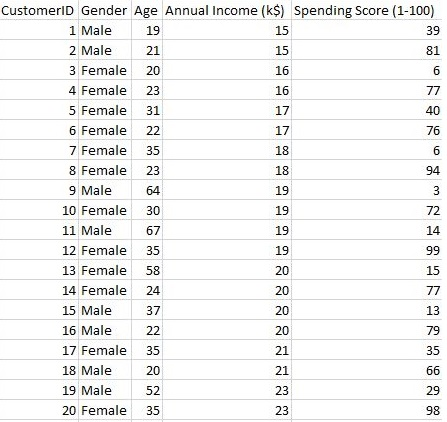
\includegraphics[scale=0.9]{mall_customers_asli}
	\caption{Dua puluh baris pertama \textit{dataset} \textit{mall\_customers} asli}
	\label{fig:mall_customers_asli}
\end{figure}

\begin{figure}
	\centering
	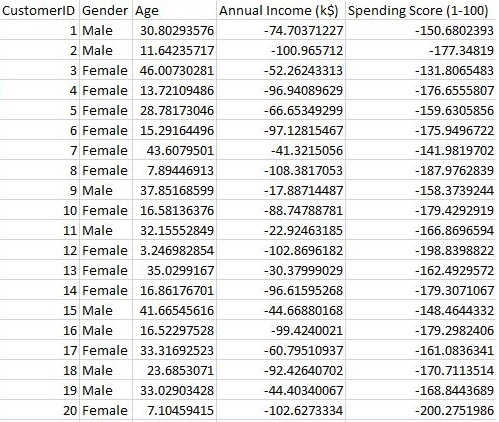
\includegraphics[scale=0.9]{rotated_mall_customers}
	\caption{Dua puluh baris pertama \textit{dataset} \textit{mall\_customers} setelah diacak}
	\label{fig:rotated_mall_customers}
\end{figure}

\subsection{Teknik \textit{Random Projection Perturbation}}
\label{subsec:rpp-fungsional}

Pengujian teknik \textit{Random Projection Perturbation} akan menggunakan \textit{dataset} \textit{mobile\_sensor}\footnote{https://www.kaggle.com/uciml/human-activity-recognition-with-smartphones} yang berisi data sensor \textit{smartphone} banyak orang yang sedang melakukan aktivitas tertentu yaitu berdiri, duduk, berbaring, berjalan, berjalan menanjak, berjalan menurun. \textit{Dataset} ini memiliki 561 buah fitur dan sebuah label. Seluruh fitur tersebut akan diacak dan diharapkan hasilnya akan mengacak \textit{dataset} sehingga nilai tiap fitur tersebut berbeda dari aslinya. \textit{Dataset} yang telah diacak juga diharapkan masih dapat diterapkan teknik penambangan data dengan hasil yang kualitasnya mirip dengan \textit{dataset} asli, pengujian untuk hal ini akan dilakukan pada bagian berikutnya yaitu pada pengujian eksperimental.

Label pada \textit{dataset} \textit{mobile\_sensor} yang ingin diacak harus dihilangkan terlebih dahulu agar hanya fitur (bersifat numerik) pada \textit{dataset} tersebut saja yang teracak. Nilai variabel \textit{epsilon} yang dipilih pada pengujian ini adalah sebesar 0.52 dan dengan nilai variabel \textit{epsilon} tersebut nilai minimal variabel \textit{k} adalah sebesar 418.0905. Pada pengujian ini perangkat lunak berhasil menghitung dengan benar nilai minimal variabel \textit{k} yaitu sebesar 418 dengan \textit{dataset} \textit{mobile\_sensor} dan nilai variabel \textit{epsilon} sebesar 0.52. Dapat dilihat Persamaan~\ref{eq:mink} adalah contoh perhitungan manual rumus nilai minimal variabel \textit{k} dengan nilai variabel \textit{epsilon} sebesar 0.52 dan jumlah baris pada \textit{dataset} sebanyak 10299 baris.
\begin{align}
	k &= \frac{4\ln{n}}{\frac{\epsilon^{2}}{2}-\frac{\epsilon^{3}}{3}} \label{eq:mink} \\
	&= \frac{4\ln{10299}}{\frac{0.52^{2}}{2}-\frac{0.52^{3}}{3}} \nonumber \\
	&= \frac{36.9592}{0.1352-0.0468} \nonumber \\
	&= 418.0905 \nonumber
\end{align}
Pada teknik \textit{Random Projection Perturbation} untuk memproyeksikan sebuah \textit{dataset} diperlukan sebuah matriks proyeksi acak. Perangkat lunak diharapkan dapat membuat sebuah matriks proyeksi acak dan menyimpannya ke dalam sebuah dokumen \textit{comma-separated values}. \textit{Dataset} \textit{mobile\_sensor} memiliki 561 buah fitur yang akan diacak dan sesuai dengan nilai minimal vaiabel \textit{k} yang sudah dihitung sebelumnya yaitu sebesar 418 maka ditentukan nilai \textit{k} yang dipakai pada pengujian ini adalah sebesar 427. Oleh karena itu, matriks proyeksi acak yang dibuat perangkat lunak seharusnya berukuran \(427\times427\).

Pada pengujian yang dilakukan, perangkat lunak berhasil membuat matriks proyeksi acak tersebut dengan ukuran yang benar dan menyimpannya pada sebuah dokumen \textit{comma-separated values} yang 10 kolom pertama pada 20 baris pertamanya dapat dilihat pada Gambar~\ref{fig:mobile_sensor_projection_matrix}. Matriks proyeksi ini akan digunakan untuk menerapkan teknik \textit{Random Projection Perturbation} terhadap \textit{dataset} \textit{mobile\_sensor}. Perangkat lunak juga berhasil menggunakan ulang matriks yang telah disimpan tersebut untuk menerapkan teknik \textit{Random Projection Perturbation} terhadap \textit{dataset} \textit{mobile\_sensor} dan hasilnya sama persis seperti hasil yang pertama kali. Matriks proyeksi tersebut juga dapat digunakan untuk data \textit{mobile\_sensor} yang lain dengan syarat masih memiliki jumlah fitur yang sama dan dengan penambahan data tersebut, nilai minimal variabel \textit{k} harus tetap lebih kurang atau sama dengan nilai \textit{k} yang dipilih. Persyaratan tersebut didasarkan oleh sifat pada teknik \textit{Random Projection Perturbation} yaitu nilai minimal variabel \textit{k} berbanding lurus dengan banyaknya objek data pada \textit{dataset} yang ingin diacak.

\begin{figure}
	\centering
	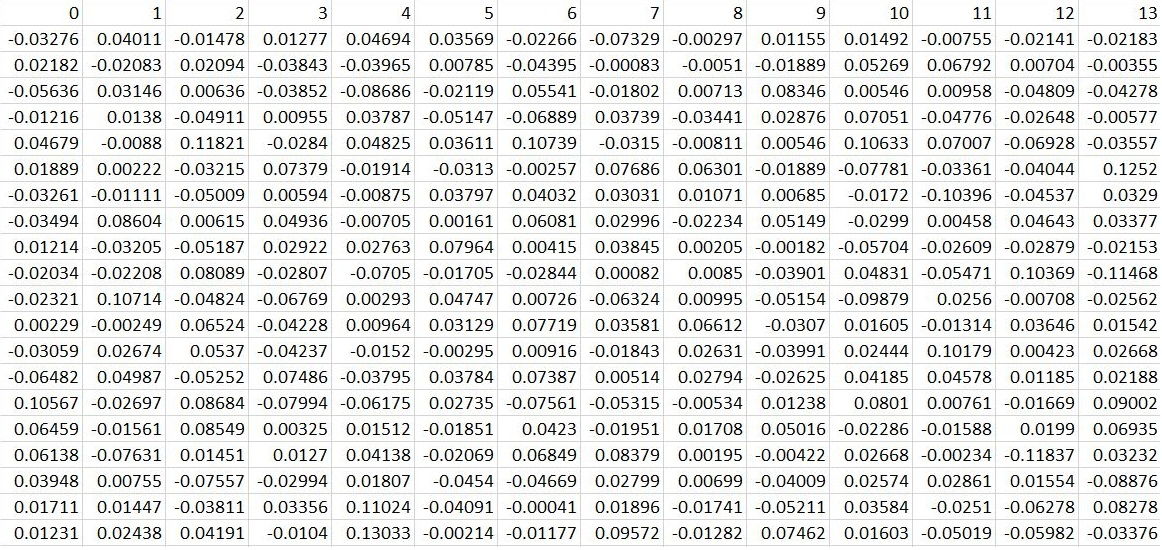
\includegraphics[scale=0.45]{mobile_sensor_projection_matrix}
	\caption{Matriks proyeksi acak yang dibuat perangkat lunak dan disimpan pada sebuah dokumen  \textit{comma-separated values}}
	\label{fig:mobile_sensor_projection_matrix}
\end{figure}

Berikut akan ditampilkan 7 fitur terakhir serta label pada 20 baris pertama \textit{dataset} asli dan \textit{dataset} yang telah diacak masing-masing pada Gambar~\ref{fig:mobile_sensor_asli} dan Gambar~\ref{fig:projected_mobile_sensor}. Dapat dilihat pada gambar tersebut, \textit{dataset} setelah diacak memiliki nilai yang berbeda dengan aslinya. Terlebih lagi setiap fitur pada \textit{dataset} yang telah diacak tidak diketahui arti dari setiap fitur tersebut apa karena sudah tereduksi sehingga seluruh fitur pada \textit{dataset} asli tercampur secara acak dan terproyeksikan ke dalam 427 fitur yang ada pada \textit{dataset} yang telah diacak. Dalam rangka untuk memastikan perangkat lunak berhasil dengan benar menerapkan teknik \textit{Random Projection Perturbation} dengan matriks proyeksi acak yang sebelumnya sudah dibuat dan disimpan oleh perangkat lunak, perhitungan manual dilakukan terhadap \textit{dataset} \textit{mobile\_sensor} dengan menggunakan matriks proyeksi tersebut. Hasil akhir dari perangkat lunak sama persis dengan hasil dari perhitungan manual. Oleh karena itu, dapat disimpulkan bahwa perangkat lunak sudah berfungsi dengan baik dan benar dalam menerapkan teknik \textit{Random Projection Perturbation}.

\begin{figure}
	\centering
	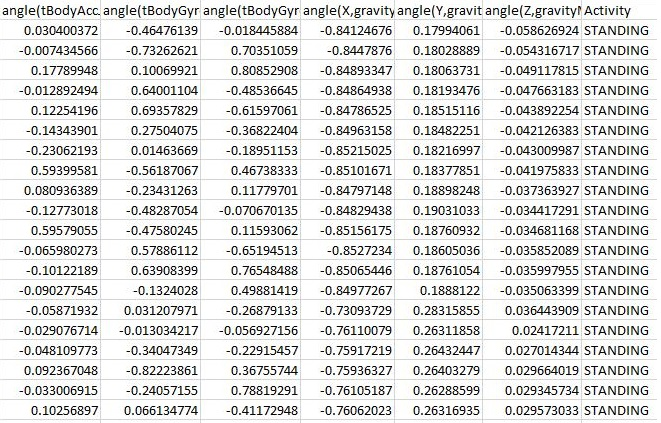
\includegraphics[scale=0.9]{mobile_sensor_asli}
	\caption{Dua puluh baris terakhir \textit{dataset} \textit{mobile\_sensor} yang asli}
	\label{fig:mobile_sensor_asli}
\end{figure}

\begin{figure}
	\centering
	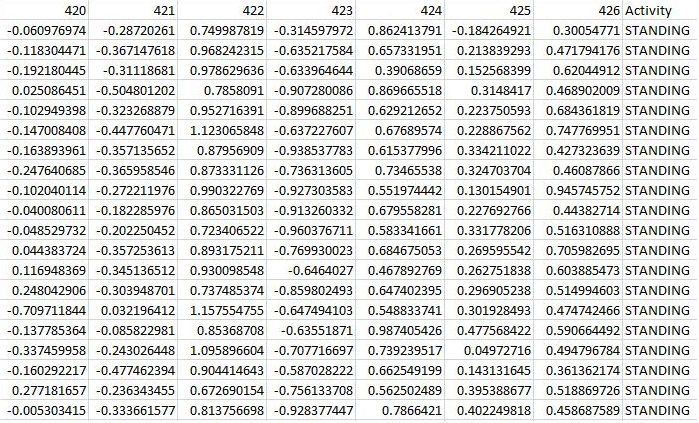
\includegraphics[scale=0.8]{projected_mobile_sensor}
	\caption{Dua puluh baris terakhir \textit{dataset} \textit{mobile\_sensor} setelah diacak}
	\label{fig:projected_mobile_sensor}
\end{figure}

Dalam rangka memastikan lebih lagi apakah perangkat lunak menerapkan teknik \textit{Random Projection Perturbation} dengan akurat, perangkat lunak pengujian dibuat untuk menguji jarak Euclidean dari setiap titik pada \textit{dataset} terhadap setiap titik lainnya. Pengujian dilakukan dengan menggunakan pertidaksamaan rentang jarak Euclidean berikut untuk menguji apakah jarak Euclidean pada \textit{dataset} yang telah diacak mempunyai distorsi yang lebih besar dari harapan pengguna. Hasil dari perangkat lunak diharapkan (\textit{dataset} yang telah diacak) memenuhi Pertidaksamaan~\ref{eq:epsilon}.

\begin{equation}\label{eq:epsilon}
	(1-eps)||u - v||^{2}<||p(u) - p(v)||^{2}<(1+eps)||u - v||^{2}
\end{equation}

Pada pengujian ini, dengan nilai variabel \textit{epsilon} sebesar 0.52 Pertidaksamaan~\ref{eq:epsilon} terpenuhi pada seluruh objek data yang ada pada \textit{dataset}. Ada salah satu kasus saat Pertidaksamaan~\ref{eq:epsilon} tidak terpenuhi yaitu apabila nilai variabel \textit{epsilon} ditentukan sebesar 0.4. Salah satu jarak Euclidean yang melanggar Pertidaksamaan~\ref{eq:epsilon} adalah baris 473 dengan baris 1306 yang memiliki jarak Euclidean sebesar 8.167734238223167 pada \textit{dataset} asli dan 9.723888530285468 pada \textit{dataset} yang telah diacak. Pengujian ini membuktikan bahwa perangkat lunak berhasil menerapkan teknik \textit{Random Projection Perturbation} dengan akurat sesuai batas distorsi yang ditentukan pengguna.

\section{Pengujian Eksperimental}
\label{sec:pengujianeksperimental}

Pengujian eksperimental bertujuan untuk menguji kualitas hasil dari perangkat lunak \textit{Randomization} pada kedua teknik \textit{Randomization} dan membandingkan kualitas hasil pengacakan dari kedua teknik tersebut pada penambangan data. Pengujian dibagi menjadi beberapa bagian seperti berikut.

\begin{enumerate}
	\item Properti Data
	\begin{enumerate}
		\item \textit{Random Rotation Perturbation} dengan \textit{dataset} \textit{diabetes}
		\item \textit{Random Projection Perturbation} dengan \textit{dataset} \textit{mobile\_sensor}
	\end{enumerate}
	\item Penambangan Data Klasifikasi
	\begin{enumerate}
		\item \textit{Random Rotation Perturbation} dengan \textit{dataset} \textit{diabetes}
		\item \textit{Random Projection Perturbation} dengan \textit{dataset} \textit{mobile\_sensor}
	\end{enumerate}
	\item Penambangan Data \textit{Clustering}
	\begin{enumerate}
		\item \textit{Random Rotation Perturbation} dengan \textit{dataset} \textit{mall\_customers}
		\item \textit{Random Projection Perturbation} dengan \textit{dataset} \textit{mobile\_sensor}
	\end{enumerate}
	\item Kesimpulan Akhir Pengujian Eksperimental
\end{enumerate}

Pengujian akan dilakukan dengan menggunakan program pengujian yang menerapkan teknik penambangan data yang telah dibuat pada bahasa pemograman Python dan didukung oleh perangkat lunak \textit{Spyder} untuk menampilkan visualisasi hasil penambangan data.

\subsection{Properti Data}
\label{subsec:pengujian-properti}

Pengujian properti data bertujuan untuk membandingkan beberapa properti pada data yaitu rata-rata, standar deviasi, nilai terkecil dan terbesar pada sebuah kolom, kuartil bawah, kuartil tengah dan kuartil atas. Pengujian ini akan membandingkan properti data pada \textit{dataset} asli dan \textit{dataset} yang telah diacak. Pengujian akan dibagi menjadi 2 bagian yaitu \textit{dataset} yang diacak dengan teknik \textit{Random Rotation Perturbation} dan \textit{dataset} yang diacak dengan teknik \textit{Random Projection Perturbation}. Berikut pengujian yang telah dilakukan.

\subsubsection{\textit{Random Rotation Perturbation}}
\label{subsubsec:pengujian-properti-rrp}

Pengujian teknik \textit{Random Rotation Perturbation} untuk membandingkan properti data akan dilakukan dengan \textit{dataset} \textit{diabetes}\footnote{https://www.kaggle.com/uciml/pima-indians-diabetes-database} yang dapat dilihat 20 baris pertamanya pada Gambar~\ref{fig:diabetes_asli}. \textit{Dataset} ini diacak dengan teknik \textit{Random Rotation Perturbation} dan hasil pengacakan dapat dilihat pada Gambar~\ref{fig:rotated_diabetes}.

\begin{figure}
	\centering
	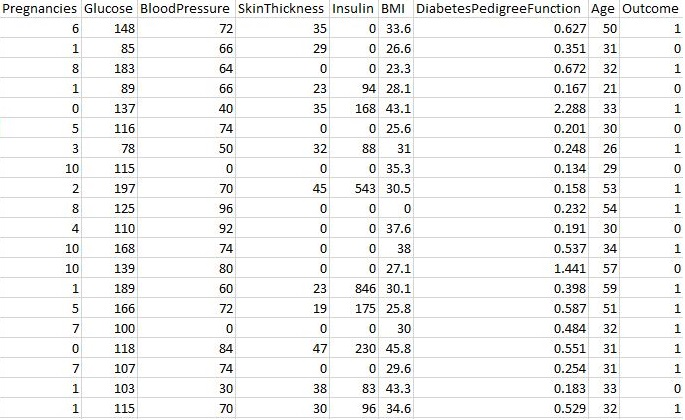
\includegraphics[scale=0.9]{diabetes_asli}
	\caption{Dua puluh baris pertama \textit{dataset} \textit{diabetes} asli}
	\label{fig:diabetes_asli}
\end{figure}

\begin{figure}
	\centering
	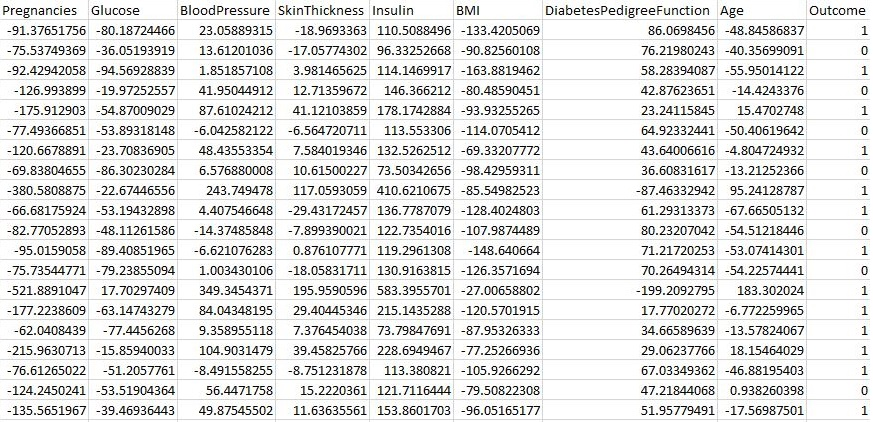
\includegraphics[scale=0.71]{rotated_diabetes}
	\caption{Dua puluh baris pertama \textit{dataset} \textit{diabetes} setelah diacak}
	\label{fig:rotated_diabetes}
\end{figure}

Properti-properti 4 kolom terakhir pada \textit{dataset} \textit{diabetes} asli dapat dilihat pada Tabel~\ref{table:properti-diabetes-asli}. Sementara untuk \textit{dataset} \textit{diabetes} yang telah diacak dapat dilihat pada Tabel~\ref{table:properti-diabetes-randomisasi}. Jika dilihat pada kedua tabel tersebut, seluruh properti pada \textit{dataset} yang telah diacak mempunyai nilai yang berbeda kecuali jumlah baris (\textit{count}) dan kolom label (\textit{Outcome}). Hal ini menunjukkan selain nilai pada setiap data, teknik \textit{Random Rotation Perturbation} juga mengacak bermacam properti data seperti rata-rata, standar deviasi, nilai terkecil dan terbesar pada sebuah kolom, kuartil bawah, kuartil tengah dan kuartil atas.
	
\begin{table}
	\centering
	\caption{Properti-properti pada \textit{dataset} \textit{diabetes} asli}
	\begin{tabular}{l|llll}
		\hline
			& \textbf{BMI} & \textbf{DiabetesPedigreeFunction} & \textbf{Age} & \textbf{Outcome} \\ \hline
		\textbf{count} & 768.000000 & 768.000000 & 768.000000 & 768.000000 \\
		\textbf{mean} & 31.992578 & 0.471876 & 33.240885 & 0.348958 \\
		\textbf{std} & 7.884160 & 0.331329 & 11.760232 & 0.476951 \\
		\textbf{min} & 0.000000 & 0.078000 & 21.000000 & 0.000000 \\
		\textbf{25\%} & 27.300000 & 0.243750 & 24.000000 & 0.000000\\
		\textbf{50\%} & 32.000000 & 0.372500 & 29.000000 & 0.000000 \\
		\textbf{75\%} & 36.600000 & 0.626250 & 41.000000 & 1.000000 \\
		\textbf{max} & 67.100000 & 2.420000 & 81.000000 & 1.000000 \\
		\hline
	\end{tabular}
	\label{table:properti-diabetes-asli}
\end{table}

\begin{table}
	\centering
	\caption{Properti-properti pada \textit{dataset} \textit{diabetes} yang telah diacak}
	\begin{tabular}{l|llll}
		\hline
		& \textbf{BMI} & \textbf{DiabetesPedigreeFunction} & \textbf{Age} & \textbf{Outcome} \\ \hline
		\textbf{count} & 768.000000 & 768.000000 & 768.000000 & 768.000000 \\
		\textbf{mean} & -103.101329 & 50.477502 & -23.129061 & 0.348958 \\
		\textbf{std} & 24.146554 & 35.533157 & 32.695887 & 0.476951  \\
		\textbf{min} & -176.332307 & -199.209279 & -74.182020 & 0.000000 \\
		\textbf{25\%} & -116.872237 & 35.049918 & -46.748389 & 0.000000 \\
		\textbf{50\%} & -101.458852 & 58.320138 & -28.463990 & 0.000000 \\
		\textbf{75\%} & -86.757613 & 73.320823 & -9.757361 & 1.000000 \\
		\textbf{max} & -22.156712 & 116.151884 & 183.302024 & 1.000000 \\
		\hline
	\end{tabular}
	\label{table:properti-diabetes-randomisasi}
\end{table}

\subsubsection{\textit{Random Projection Perturbation}}
\label{subsubsec:pengujian-properti-rpp}

Pengujian teknik \textit{Random Projection Perturbation} untuk membandingkan properti data akan dilakukan dengan \textit{dataset} \textit{mobile\_sensor} yang dapat dilihat 20 baris pertamanya pada Gambar~\ref{fig:mobile_sensor_asli}. \textit{Dataset} ini diacak dengan teknik \textit{Random Projection Perturbation} dan hasil pengacakan dapat dilihat pada Gambar~\ref{fig:projected_mobile_sensor}.

Properti-properti 4 buah kolom pada \textit{dataset} \textit{mobile\_sensor} asli dapat dilihat pada Tabel~\ref{table:properti-mobile-sensor-asli}. Sementara untuk \textit{dataset} \textit{mobile\_sensor} yang telah diacak dapat dilihat pada Tabel~\ref{table:properti-mobile-sensor-randomisasi}. Jika dilihat pada kedua tabel tersebut, seluruh properti pada \textit{dataset} yang telah diacak mempunyai nilai yang berbeda kecuali jumlah baris (\textit{count}). Hal ini menunjukkan selain nilai pada setiap data, teknik \textit{Random Projection Perturbation} juga mengacak bermacam properti \textit{dataset} seperti rata-rata, standar deviasi, nilai terkecil dan terbesar pada sebuah kolom, kuartil bawah, kuartil tengah dan kuartil atas.

\begin{table}
	\centering
	\caption{Properti-properti pada \textit{dataset} \textit{mobile\_sensor} asli}
	\begin{tabular}{l|llll}
		\hline
			& tBodyAcc-mean()-X & tBodyAcc-mean()-Y & angle(Y,gravityMean) & angle(Z,gravityMean)\\ \hline
		\textbf{count} & 10299.000000 & 10299.000000 & 10299.000000 & 10299.000000 \\
		\textbf{mean} & 0.274347 & -0.017743 & 0.063255 & -0.054284 \\
		\textbf{std} & 0.067628 & 0.037128 & 0.305468 & 0.268898 \\
		\textbf{min} & -1.000000 & -1.000000 & -1.000000 & -1.000000 \\
		\textbf{25\%} & 0.262625 & -0.024902 & 0.002151 & -0.131880 \\
		\textbf{50\%} & 0.277174 & -0.017162 & 0.182028 & -0.003882 \\
		\textbf{75\%} & 0.288354 & -0.010625 & 0.250790 & 0.102970 \\
		\textbf{max} & 1.000000 & 1.000000 & 1.000000 & 1.000000 \\
		\hline
	\end{tabular}
	\label{table:properti-mobile-sensor-asli}
\end{table}

\begin{table}
	\centering
	\caption{Properti-properti pada \textit{dataset} \textit{mobile\_sensor} yang telah diacak}
	\begin{tabular}{l|llll}
		\hline
		& 0 & 1 & 425 & 426 \\ \hline
		\textbf{count} & 10299.000000 & 10299.000000 & 10299.000000 & 10299.000000 \\
		\textbf{mean} & 0.136942 & -0.289681 & 0.173610 & 0.353280 \\
		\textbf{std} & 0.528322 & 0.266849 & 0.214992 & 0.475443 \\
		\textbf{min} & -1.433025 & -1.206428 & -1.437424 & -0.976616 \\
		\textbf{25\%} & -0.340174 & -0.482918 & 0.033424 & -0.049233 \\
		\textbf{50\%} & 0.308314 & -0.270461 & 0.179048 & 0.322172 \\
		\textbf{75\%} & 0.582374 & -0.097266 & 0.325611 & 0.688616 \\
		\textbf{max} & 1.283867 & 0.726498 & 0.978304 & 1.786145 \\
		\hline
	\end{tabular}
	\label{table:properti-mobile-sensor-randomisasi}
\end{table}

\subsubsection{Kesimpulan}
\label{subsubsec:pengujian-properti-kesimpulan}

Berdasarkan pengujian properti data pada \textit{dataset} asli, \textit{dataset} yang telah diacak menggunakan teknik \textit{Random Rotation Perturbation}, dan \textit{dataset} yang telah diacak menggunakan teknik \textit{Random Projection Perturbation} dibuat kesimpulan sekaligus membandingkan antara kedua teknik \textit{Randomization}. Pada Tabel~\ref{table:perbandingan-properti} dapat dilihat hasil akhir pengujian antara properti data pada \textit{dataset} asli dan \textit{dataset} yang telah diacak dengan \textit{Random Rotation Perturbation} dan \textit{Random Projection Perturbation}. Dapat dilihat pada tabel tersebut metode \textit{Randomization} mengacak data dengan baik dan tidak menjaga properti-properti lain pada data selain jarak Euclidean.

\begin{table}
	\centering
	\caption{Perbandingan Properti Data}
	\begin{tabular}{|l|l|l|}
		\hline
		& \textbf{\textit{Rotation}} & \textbf{\textit{Projection}} \\ \hline
		\textbf{Rata-rata} & Berbeda & Berbeda \\
		\textbf{Standar Deviasi} & Berbeda & Berbeda \\
		\textbf{Nilai Terkecil} & Berbeda & Berbeda \\
		\textbf{Nilai Terbesar} & Berbeda & Berbeda \\
		\textbf{Kuartil Bawah} & Berbeda & Berbeda \\
		\textbf{Kuartil Tengah} & Berbeda & Berbeda \\
		\textbf{Kuartil Atas} & Berbeda & Berbeda \\
		\hline
	\end{tabular}
	\label{table:perbandingan-properti}
\end{table}

\subsection{Penambangan Data Klasifikasi}
\label{subsec:pengujian-klasifikasi}
Pengujian dengan penambangan data klasifikasi akan berpusat pada pembuatan model dengan \textit{dataset} asli dan \textit{dataset} yang telah diacak dan membandingkan kedua model tersebut. Teknik penambangan data klasifikasi yang digunakan adalah \textit{k-nearest neighbors}. Pengujian dengan penambangan data klasifikasi akan dibagi menjadi 2 bagian yaitu \textit{dataset} yang diacak dengan teknik \textit{Random Rotation Perturbation} dan \textit{dataset} yang diacak dengan teknik \textit{Random Projection Perturbation}. Pengujian akan membandingkan beberapa informasi pada \textit{dataset} asli dan \textit{dataset} yang telah diacak. Beberapa informasi tersebut dijabarkan sebagai berikut.
\begin{enumerate}
	\item Akurasi model \textit{k-nearest neighbors}
	\item Nilai variabel \textit{k} yang modelnya memiliki akurasi tertinggi
	\item Waktu eksekusi pelatihan model dan prediksi dengan model yang telah dibuat
\end{enumerate}
Tujuan dari pengujian ini adalah mencari informasi yang masih terjaga (mempunyai hasil yang sama atau mirip) antara model yang dilatih dengan \textit{dataset} asli dan \textit{dataset} yang telah diacak.

\subsubsection{\textit{Random Rotation Perturbation}}
\label{subsubsec:pengujian-klasifikasi-rrp}

Pengujian teknik \textit{Random Rotation Perturbation} untuk penambangan data klasifikasi dengan algoritma \textit{k-nearest neighbors} akan dilakukan dengan \textit{dataset} \textit{diabetes} yang dapat dilihat 20 baris pertamanya pada Gambar~\ref{fig:diabetes_asli}. \textit{Dataset} ini diacak dengan teknik \textit{Random Rotation Perturbation} dan hasil pengacakan dapat dilihat pada Gambar~\ref{fig:rotated_diabetes}. Dengan kedua \textit{dataset} tersebut, dilakukan penambangan data terhadap kedua \textit{dataset} tersebut dan dihasilkan berbagai macam informasi yang dapat dibandingkan. Berikut adalah hasil pengujian dan penjelasannya.

Teknik penambangan data \textit{k-nearest neighbors} diterapkan menggunakan 8 buah fitur yang ada untuk menguji apakah \textit{dataset} asli dan \textit{dataset} yang telah diacak mempunyai akurasi model klasifikasi yang sama persis. Pengujian tersebut didasarkan pada sifat dari teknik \textit{Random Rotation Perturbation} yang menjamin jarak Euclidean setiap titik tidak berubah sama sekali. \textit{Dataset} akan dibagi dua menjadi \textit{train set} dan \textit{test set} yang masing-masing berguna untuk melatih model dan menghitung akurasi model. Akurasi akan dihitung pada setiap jumlah tetangga (nilai \textit{k}) dari 1 sampai 20. Implementasi kode teknik penambangan data ini diterapkan dengan bahasa pemograman Python dan dibantu oleh \textit{library} Scikit-learn. Pada Gambar~\ref{fig:plot_akurasi_diabetes} dapat dilihat grafik akurasi model \textit{k-nearest neighbors} dalam memprediksi label \textit{training set} dan \textit{test set} pada \textit{dataset} asli dan \textit{dataset} yang telah diacak. Apabila dibandingkan, kedua grafik tersebut terlihat memiliki nilai akurasi yang sama persis untuk setiap nilai \textit{k}. 

\begin{figure}
	\centering
	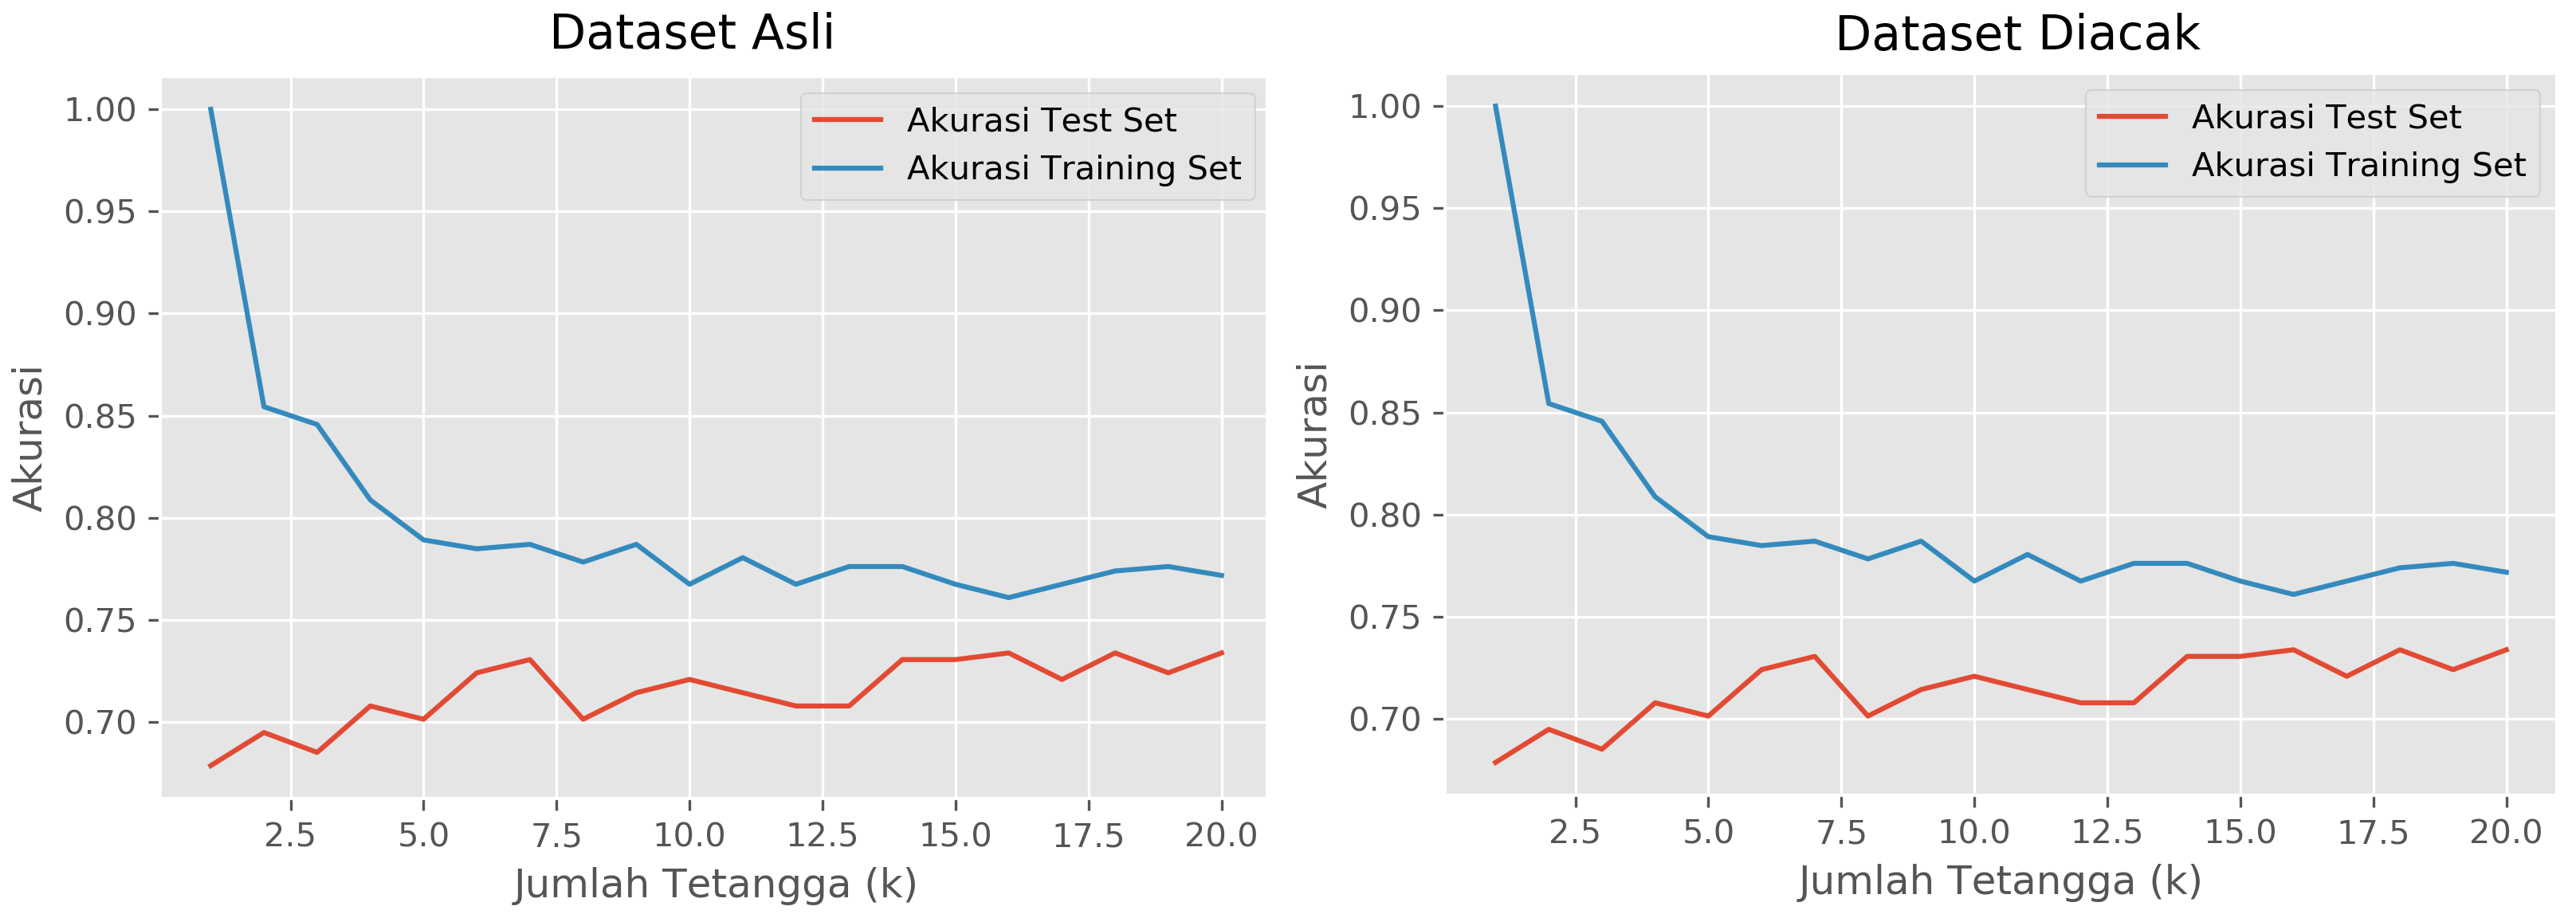
\includegraphics[scale=0.185]{plot_akurasi_diabetes}
	\caption{Grafik akurasi model klasifikasi pada \textit{training set} dan \textit{test set} \textit{dataset} \textit{diabetes}}
	\label{fig:plot_akurasi_diabetes}
\end{figure}

Akurasi model untuk setiap nilai \textit{k} dari 14 sampai 18 pada \textit{dataset} asli dan \textit{dataset} yang telah diacak dapat dilihat masing-masing pada Listing~\ref{diabetes_akurasi_asli} dan Listing~\ref{diabetes_akurasi_randomisasi}. Akurasi tertinggi pada model \textit{k-nearest neighbors} dengan \textit{dataset} asli adalah sebesar 0.7337662337662337 dengan nilai \textit{k} sebesar 16. Nilai yang sama juga muncul pada \textit{dataset} yang telah diacak. Hal ini dapat menjadi bukti bahwa teknik \textit{Random Rotation Perturbation} menjaga jarak Euclidean dengan sempurna, tidak ada perubahan sama sekali pada jarak Euclidean antara seluruh titik. Oleh karena itu model \textit{k-nearest neighbors} yang terbuat memiliki hasil yang sama persis.

\noindent\begin{minipage}{.46\textwidth}
	\begin{lstlisting}[caption=\textit{Dataset diabetes} Asli,frame=tlrb, label=diabetes_akurasi_asli]{Name}
Akurasi setiap K pada 
training set dataset asli:
14: 0.7760869565217391
15: 0.7673913043478261
16: 0.7608695652173914
17: 0.7673913043478261
18: 0.7739130434782608

Akurasi setiap K pada 
test set dataset asli: 
14: 0.7305194805194806
15: 0.7305194805194806
16: 0.7337662337662337
17: 0.7207792207792207
18: 0.7337662337662337
	\end{lstlisting}
\end{minipage}\hfill
\begin{minipage}{.46\textwidth}
	\begin{lstlisting}[caption=\textit{Dataset diabetes} Teracak,frame=tlrb, label=diabetes_akurasi_randomisasi]{Name}
Akurasi setiap K pada training 
set dataset teracak: 
14: 0.7760869565217391
15: 0.7673913043478261
16: 0.7608695652173914
17: 0.7673913043478261
18: 0.7739130434782608

Akurasi setiap K pada test 
set dataset teracak: 
14: 0.7305194805194806
15: 0.7305194805194806
16: 0.7337662337662337
17: 0.7207792207792207
18: 0.7337662337662337
	\end{lstlisting}
\end{minipage}
	
Waktu eksekusi yang dibutuhkan untuk melatih model klasifikasi dengan nilai \textit{k} sebesar 16 memakai \textit{dataset} asli adalah sebesar 0.0009965896606445312 detik dan waktu yang dibutuhkan untuk memprediksi \textit{test set} sebesar 0.015623807907104492 detik. Sementara untuk \textit{dataset} yang telah diacak membutuhkan waktu eksekusi untuk melatih model klasifikasi sebesar 0.0009937286376953125 detik dan waktu yang dibutuhkan untuk melakukan prediksi adalah sebesar 0.01565837860107422 detik. Hal ini menunjukkan tidak ada pengaruh yang signifikan terhadap durasi waktu eksekusi untuk melatih model dan memprediksi dengan \textit{dataset} asli dan \textit{dataset} yang telah diacak.

\subsubsection{\textit{Random Projection Perturbation}}
\label{subsubsec:pengujian-klasifikasi-rpp}

Pengujian teknik \textit{Random Projection Perturbation} untuk penambangan data klasifikasi dengan algoritma \textit{k-nearest neighbors} akan dilakukan dengan \textit{dataset} \textit{mobile\_sensor} yang dapat dilihat 20 baris pertamanya pada Gambar~\ref{fig:mobile_sensor_asli}. \textit{Dataset} ini diacak dengan teknik \textit{Random Projection Perturbation} dan hasil pengacakan dapat dilihat pada Gambar~\ref{fig:projected_mobile_sensor}. Dengan kedua \textit{dataset} tersebut, dilakukan penambangan data terhadap kedua \textit{dataset} tersebut dan dihasilkan berbagai macam informasi yang dapat dibandingkan. Berikut adalah hasil pengujian dan penjelasannya.

Teknik penambangan data \textit{k-nearest neighbors} diterapkan menggunakan 561 fitur yang ada untuk menguji apakah \textit{dataset} mempunyai akurasi model klasifikasi yang hampir sama. Pengujian tersebut didasarkan pada sifat teknik \textit{Random Projection Perturbation} yang menjamin jarak Euclidean setiap titik terjaga dengan besar distorsi yang ditentukan pengguna. \textit{Dataset} akan dibagi dua menjadi \textit{train set} dan \textit{test set} yang masing-masing berguna untuk melatih model dan menghitung akurasi model. Akurasi akan dihitung dengan jumlah tetangga (nilai \textit{k}) dari 1 sampai 30. Implementasi kode teknik penambangan data ini diterapkan dengan bahasa pemograman Python dan dibantu oleh \textit{library} Scikit-learn.

Pada Gambar~\ref{fig:plot_akurasi_mobile_sensor} dapat dilihat grafik akurasi model \textit{k-nearest neighbors} dalam memprediksi label \textit{training set} dan \textit{test set} pada \textit{dataset} asli dan \textit{dataset} yang telah diacak. Apabila dibandingkan, kedua grafik tersebut memiliki nilai akurasi yang mirip. Walaupun begitu, teknik \textit{Random Projection Perturbation} tidak menjamin jarak Euclidean terjaga dengan sempurna maka ada sedikit perbedaan yang lumayan terlihat khususnya pada akurasi \textit{test set} dan nilai \textit{k} yang memiliki akurasi tertinggi. Tetapi perbedaan nilai akurasinya masih mirip dengan \textit{dataset} asli. 
	
\begin{figure}
	\centering
	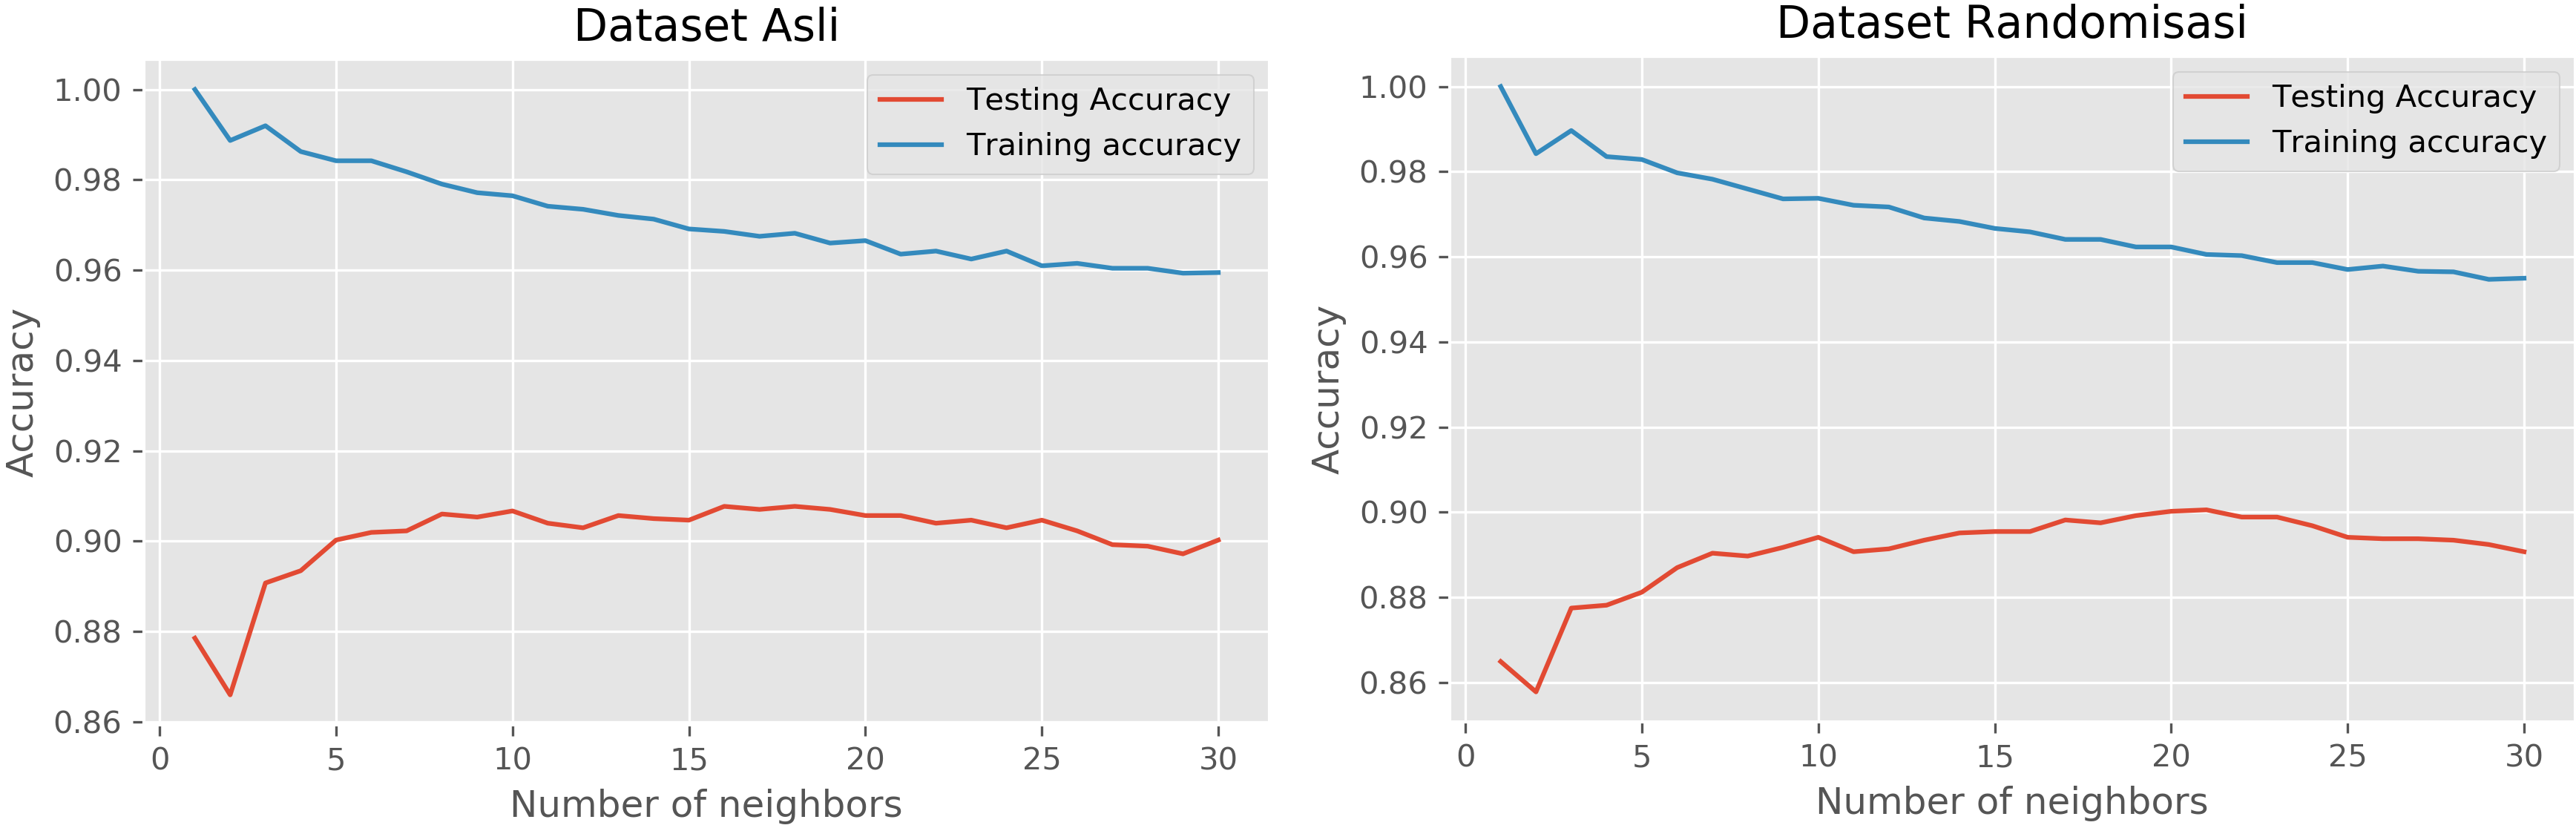
\includegraphics[scale=0.17]{plot_akurasi_mobile_sensor}
	\caption{Grafik akurasi model klasifikasi pada \textit{training set} dan \textit{test set} \textit{dataset} \textit{mobile\_sensor}}
	\label{fig:plot_akurasi_mobile_sensor}
\end{figure}

Akurasi model untuk setiap nilai \textit{k} dari 19 sampai 23 pada \textit{dataset} asli dan \textit{dataset} yang telah diacak dapat dilihat masing-masing pada Listing~\ref{mobile_sensor_akurasi_asli} dan Listing~\ref{mobile_sensor_akurasi_randomisasi}. Dapat dilihat pada kedua listing tersebut akurasi \textit{test set} pada kedua \textit{dataset} berbeda. Akurasi \textit{test set} tertinggi pada \textit{dataset} asli adalah sebesar 0.9077027485578555 dengan nilai \textit{k} sebesar 16. Sementara pada \textit{dataset} yang telah diacak, akurasi \textit{test set} tertingginya adalah sebesar 0.9005768578215134 dengan nilai \textit{k} sebesar 21. Jika dihitung perbedaan akurasinya adalah sebesar 0.0071258907363421 yang mana relatif kecil tetapi ada perbedaan pada nilai \textit{k} yang memiliki akurasi tertinggi. Dengan perbedaan akurasi yang relatif kecil dan \textit{dataset} yang telah diacak teracak dengan baik maka dapat disimpulkan bahwa teknik \textit{Random Projection Perturbation} menjaga jarak Euclidean dengan baik dan distorsinya terkontrol sesuai yang pengguna inginkan. Oleh karena itu, model \textit{k-nearest neighbors} yang terbuat memiliki hasil yang sangat mirip.
	
\noindent\begin{minipage}{.46\textwidth}
	\begin{lstlisting}[caption=\textit{Dataset mobile\_sensor} Asli,frame=tlrb, label=mobile_sensor_akurasi_asli]{Name}
Akurasi setiap K pada 
training set dataset asli: 
19: 0.9659956474428727
20: 0.9665397170837867
21: 0.9635473340587595
22: 0.9642274211099021
23: 0.9624591947769314

Akurasi setiap K pada 
test set dataset asli: 
19: 0.9070240922972514
20: 0.9056667797760435
21: 0.9056667797760435
22: 0.9039701391245334
23: 0.9046487953851374
	\end{lstlisting}
	\end{minipage}\hfill
	\begin{minipage}{.46\textwidth}
	\begin{lstlisting}[caption=\textit{Dataset mobile\_sensor} Teracak,frame=tlrb, label=mobile_sensor_akurasi_randomisasi]{Name}
Akurasi setiap K pada training 
set dataset teracak: 
19: 0.9623231773667029
20: 0.9623231773667029
21: 0.9605549510337323
22: 0.9602829162132753
23: 0.9586507072905331

Akurasi setiap K pada test 
set dataset teracak: 
19: 0.8992195453003053
20: 0.9002375296912114
21: 0.9005768578215134
22: 0.8988802171700034
23: 0.8988802171700034
	\end{lstlisting}
\end{minipage}

Waktu eksekusi yang dibutuhkan untuk melatih model klasifikasi dengan nilai \textit{k} sebesar 16 memakai \textit{dataset} asli adalah sebesar 0.2872335910797119 detik dan waktu yang dibutuhkan untuk memprediksi \textit{test set} sebesar 17.754546642303467 detik. Sementara untuk \textit{dataset} yang telah diacak membutuhkan waktu eksekusi untuk melatih model klasifikasi dengan nilai \textit{k} sebesar 21 adalah 0.5630350112915039 detik detik dan waktu yang dibutuhkan untuk melakukan prediksi adalah sebesar 12.86760687828064 detik. Pada \textit{dataset} yang telah diacak waktu prediksi lebih cepat dikarenakan fitur-fitur yang ada lebih sedikit daripada \textit{dataset} asli. Hal ini menunjukkan ada pengaruh yang signifikan terhadap durasi waktu eksekusi untuk melatih model dan memprediksi dengan \textit{dataset} asli dan \textit{dataset} yang telah diacak.

\subsubsection{Kesimpulan}
\label{subsubsec:pengujian-klasifikasi-kesimpulan}

Berdasarkan pengujian dengan teknik penambangan data klasifikasi menggunakan teknik \textit{k-nearest neighbors} pada \textit{dataset} asli, \textit{dataset} yang telah diacak menggunakan teknik \textit{Random Rotation Perturbation}, dan \textit{dataset} yang telah diacak menggunakan teknik \textit{Random Projection Perturbation} dibuat kesimpulan sekaligus membandingkan antara kedua teknik \textit{Randomization}. Pada Tabel~\ref{table:perbandingan-klasifikasi} dapat dilihat hasil akhir pengujian antara model yang dilatih dengan \textit{dataset} asli dan \textit{dataset} yang telah diacak dengan \textit{Random Rotation Perturbation} dan \textit{Random Projection Perturbation}.

\begin{table}
	\centering
	\caption{Perbandingan Model \textit{k-nearest neighbors}}
	\begin{tabular}{|l|l|l|}
		\hline
		& \textbf{\textit{Rotation}} & \textbf{\textit{Projection}} \\ \hline
		\textbf{Akurasi Model} & Sama & Sangat Mirip \\
		\textbf{\textit{k} terbaik} & Sama & Dapat Berbeda \\
		\textbf{Waktu Eksekusi} & Sama & Lebih Cepat \\
		\hline
	\end{tabular}
	\label{table:perbandingan-klasifikasi}
\end{table}

Akurasi model \textit{k-nearest neighbors} terjaga dengan baik pada kedua teknik \textit{Randomization} yang dikarenakan oleh jarak Euclideannya tetap terjaga setelah \textit{dataset} diacak. Tetapi untuk teknik \textit{Random Projection Perturbation} ada persyaratan yang harus dipenuhi agar jarak Euclidean dapat terjaga dengan baik dan tidak bisa sama persis dengan aslinya seperti teknik \textit{Random Rotation Perturbation}. Nilai variabel \textit{k} terbaik (memiliki akurasi tertingi) dalam pembuatan model \textit{k-nearest neighbors} sama persis pada teknik \textit{Random Rotation Perturbation}. Tetapi pada teknik \textit{Random Projection Perturbation} dapat berubah. Hal ini menyebabkan perlunya perhitungan kembali untuk menentukan nilai variabel \textit{k} yang baik untuk dipakai. Waktu eksekusi pembuatan model dan prediksi hanya memiliki perbedaan pada model yang menggunakan \textit{dataset} yang telah diacak dengan teknik \textit{Random Projection Perturbation}. Waktu eksekusinya lebih cepat dikarenakan oleh data pada \textit{dataset} lebih sedikit karenda dimensinya direduksi.

\subsection{Penambangan Data \textit{Clustering}}
\label{subsec:pengujian-clustering}

Pengujian dengan penambangan data \textit{clustering} akan berpusat pada pembuatan model \textit{clustering} dengan \textit{dataset} asli dan \textit{dataset} yang telah diacak dan membandingkan kedua model tersebut. Teknik penambangan data \textit{clustering} yang digunakan adalah \textit{k-means}. Pengujian akan membandingkan beberapa informasi pada \textit{dataset} asli dan \textit{dataset} yang telah diacak. Beberapa informasi tersebut dijabarkan sebagai berikut.
\begin{enumerate}
	\item \textit{Sum of Squared Error}
	\item \textit{Silhoutte Score}
	\item Nilai variabel \textit{k} (jumlah \textit{cluster}) yang modelnya memiliki kualitas \textit{clustering} terbaik
	\item Visualisasi \textit{cluster}
	\item Waktu eksekusi pelatihan model dan prediksi dengan model yang telah dibuat
\end{enumerate}
Tujuan dari pengujian ini adalah mencari informasi yang masih terjaga (mempunyai hasil yang sama atau mirip) antara model yang dilatih dengan \textit{dataset} asli dan \textit{dataset} yang telah diacak. Selain itu metode \textit{Adjusted Rand Index} juga digunakan untuk menghitung kemiripan antara kedua model.

\subsubsection{\textit{Random Rotation Perturbation}}
\label{subsubsec:pengujian-clustering-rrp}

Pengujian teknik \textit{Random Rotation Perturbation} untuk penambangan data \textit{clustering} dengan menggunakan algoritma \textit{k-means} akan dilakukan dengan \textit{dataset} \textit{mall\_customers} yang dapat dilihat 20 baris pertamanya pada Gambar~\ref{fig:mall_customers_asli}. \textit{Dataset} ini diacak dengan teknik \textit{Random Rotation Perturbation} dan hasil pengacakan dapat dilihat pada Gambar~\ref{fig:rotated_mall_customers}. Dengan kedua \textit{dataset} tersebut, dilakukan penambangan data terhadap kedua \textit{dataset} tersebut dan dihasilkan berbagai macam informasi yang dapat dibandingkan. Berikut adalah hasil pengujian dan penjelasannya.

Dalam menentukan jumlah \textit{cluster} atau nilai \textit{k} yang terbaik untuk membuat model \textit{clustering} dengan algoritma \textit{k-means} perlu ada metode untuk menentukan nilai tersebut. Metode Elbow menjadi salah satu metode yang digunakan untuk  menentukan nilai \textit{k} yang terbaik untuk dipakai. Pada Gambar~\ref{fig:elbow_mall_customers} terdapat grafik \textit{Sum of Squared Error} untuk menggunakan metode Elbow pada \textit{dataset} asli dan \textit{dataset} yang telah diacak. Terlihat nilai \textit{k} sebesar 5, 6, dan 7 adalah kandidat terbaik untuk menjadi nilai \textit{k} yang dipakai pada \textit{dataset} asli maupun \textit{dataset} yang telah diacak. Pada kedua \textit{dataset} tersebut grafik \textit{Sum of Squared Error}-nya terlihat sama persis dikarenakan teknik \textit{Random Rotation Perturbation} menjaga jarak Euclidean dengan sempurna. Dalam menentukan nilai \textit{k} yang terbaik antara ketiga nilai tersebut, \textit{Silhoutte Score} dapat digunakan untuk metode alternatif untuk menentukan nilai \textit{k} yang terbaik.

\begin{figure}
	\centering
	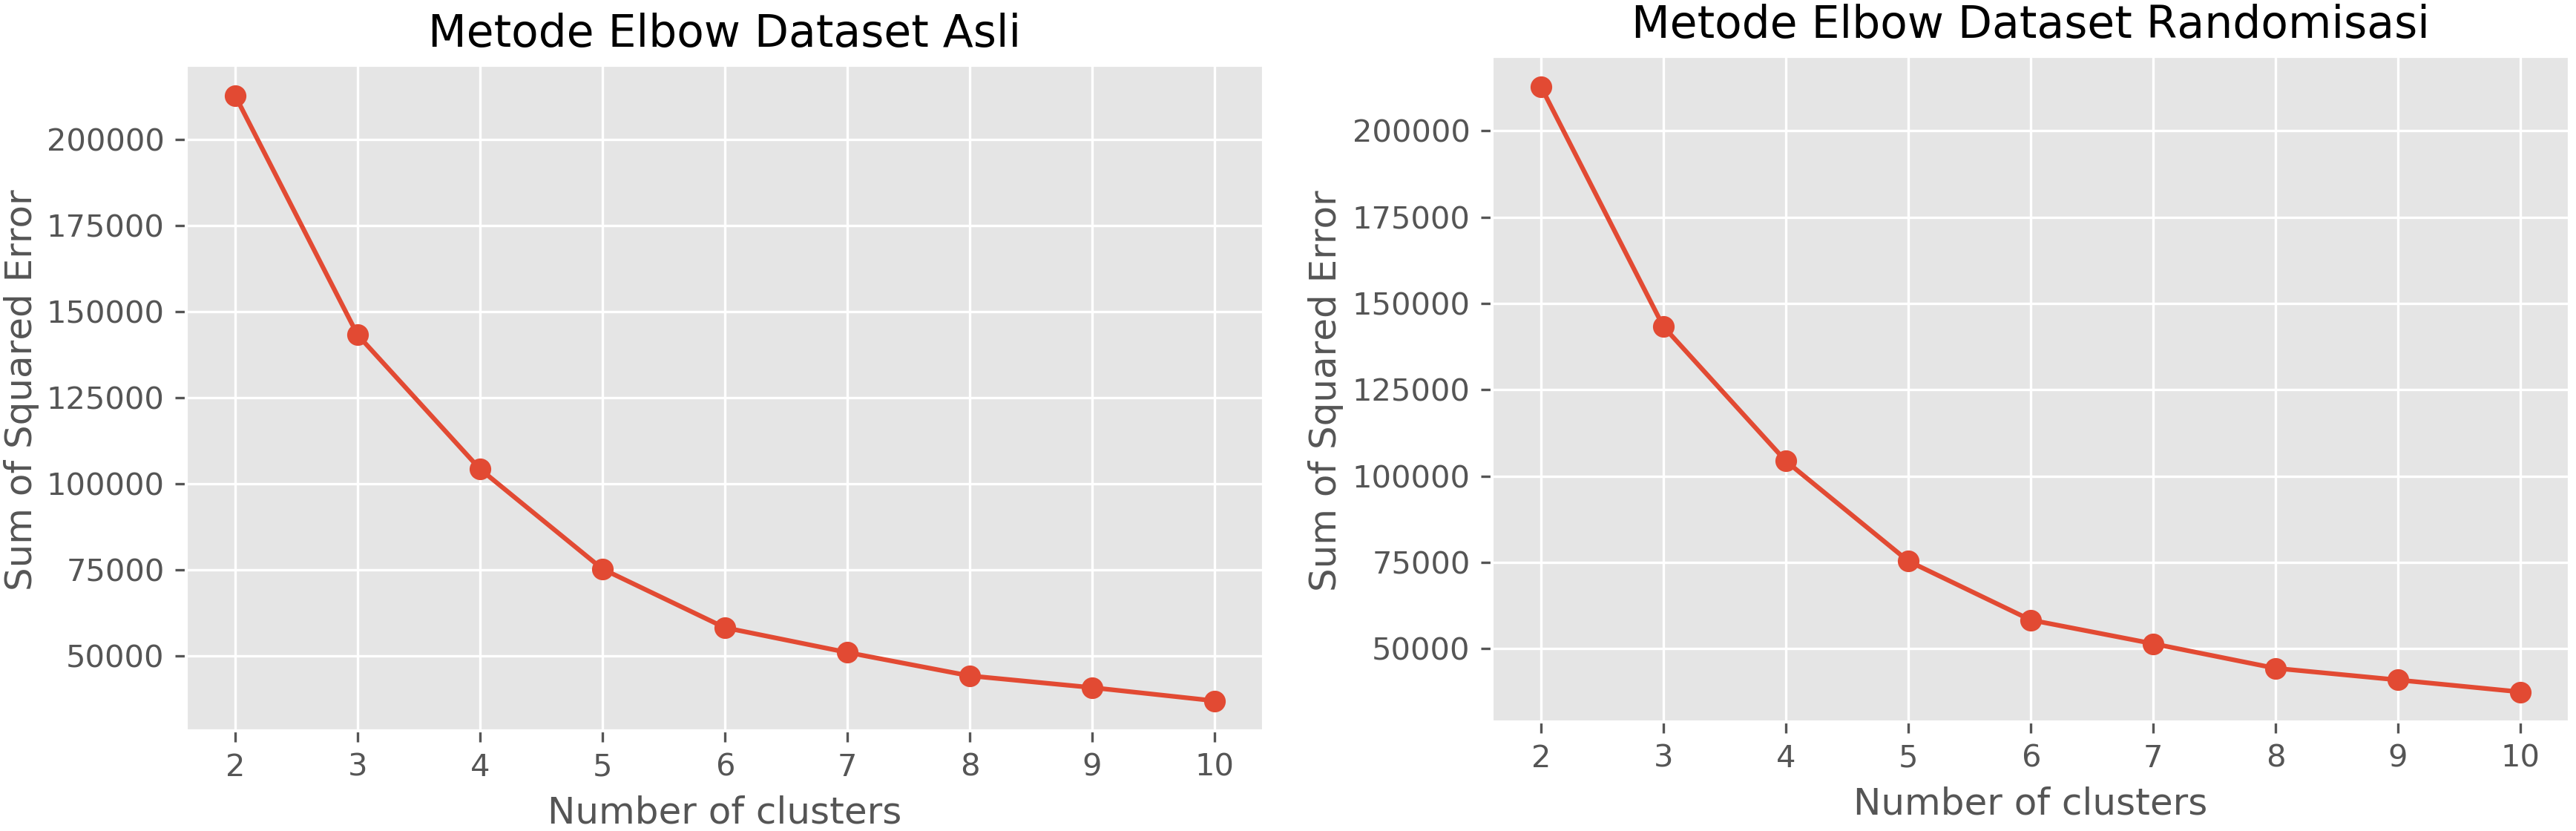
\includegraphics[scale=0.17]{elbow_mall_customers}
	\caption{Grafik \textit{Sum of Squared Error} model \textit{clustering} pada \textit{dataset} \textit{mall\_customers}}
	\label{fig:elbow_mall_customers}
\end{figure}

Pada Gambar~\ref{fig:siluet_mall_customers} terdapat grafik \textit{Silhoutte Score} dari \textit{dataset} \textit{mall\_customers} asli dan yang telah diacak. Dapat terlihat kedua grafik \textit{Silhoutte Score} terlihat sama persis dan dapat dilihat nilai-nilai pada setiap \textit{k} tersebut di Listing~\ref{mall_customers_siluet_asli} dan Listing~\ref{mall_customers_siluet_randomisasi} ada sedikit perbedaan yang tidak terlalu signifikan. Hal ini mungkin dikarenakan oleh nilai pada setiap data yang berbeda dan mempengaruhi sedikit algoritma pada \textit{Silhoutte Score}. Dapat terlihat \textit{Silhoutte Score} pada nilai \textit{k} 6 adalah nilai paling besar yaitu 0.4523443947724053 pada \textit{dataset} asli dan 0.4523443947780976 pada \textit{dataset} yang telah diacak. Hal ini menunjukkan teknik \textit{Random Rotation Perturbation} tidak mempengaruhi secara signifikan nilai \textit{Silhoutte Score} pada setiap \textit{k}.

\begin{figure}
	\centering
	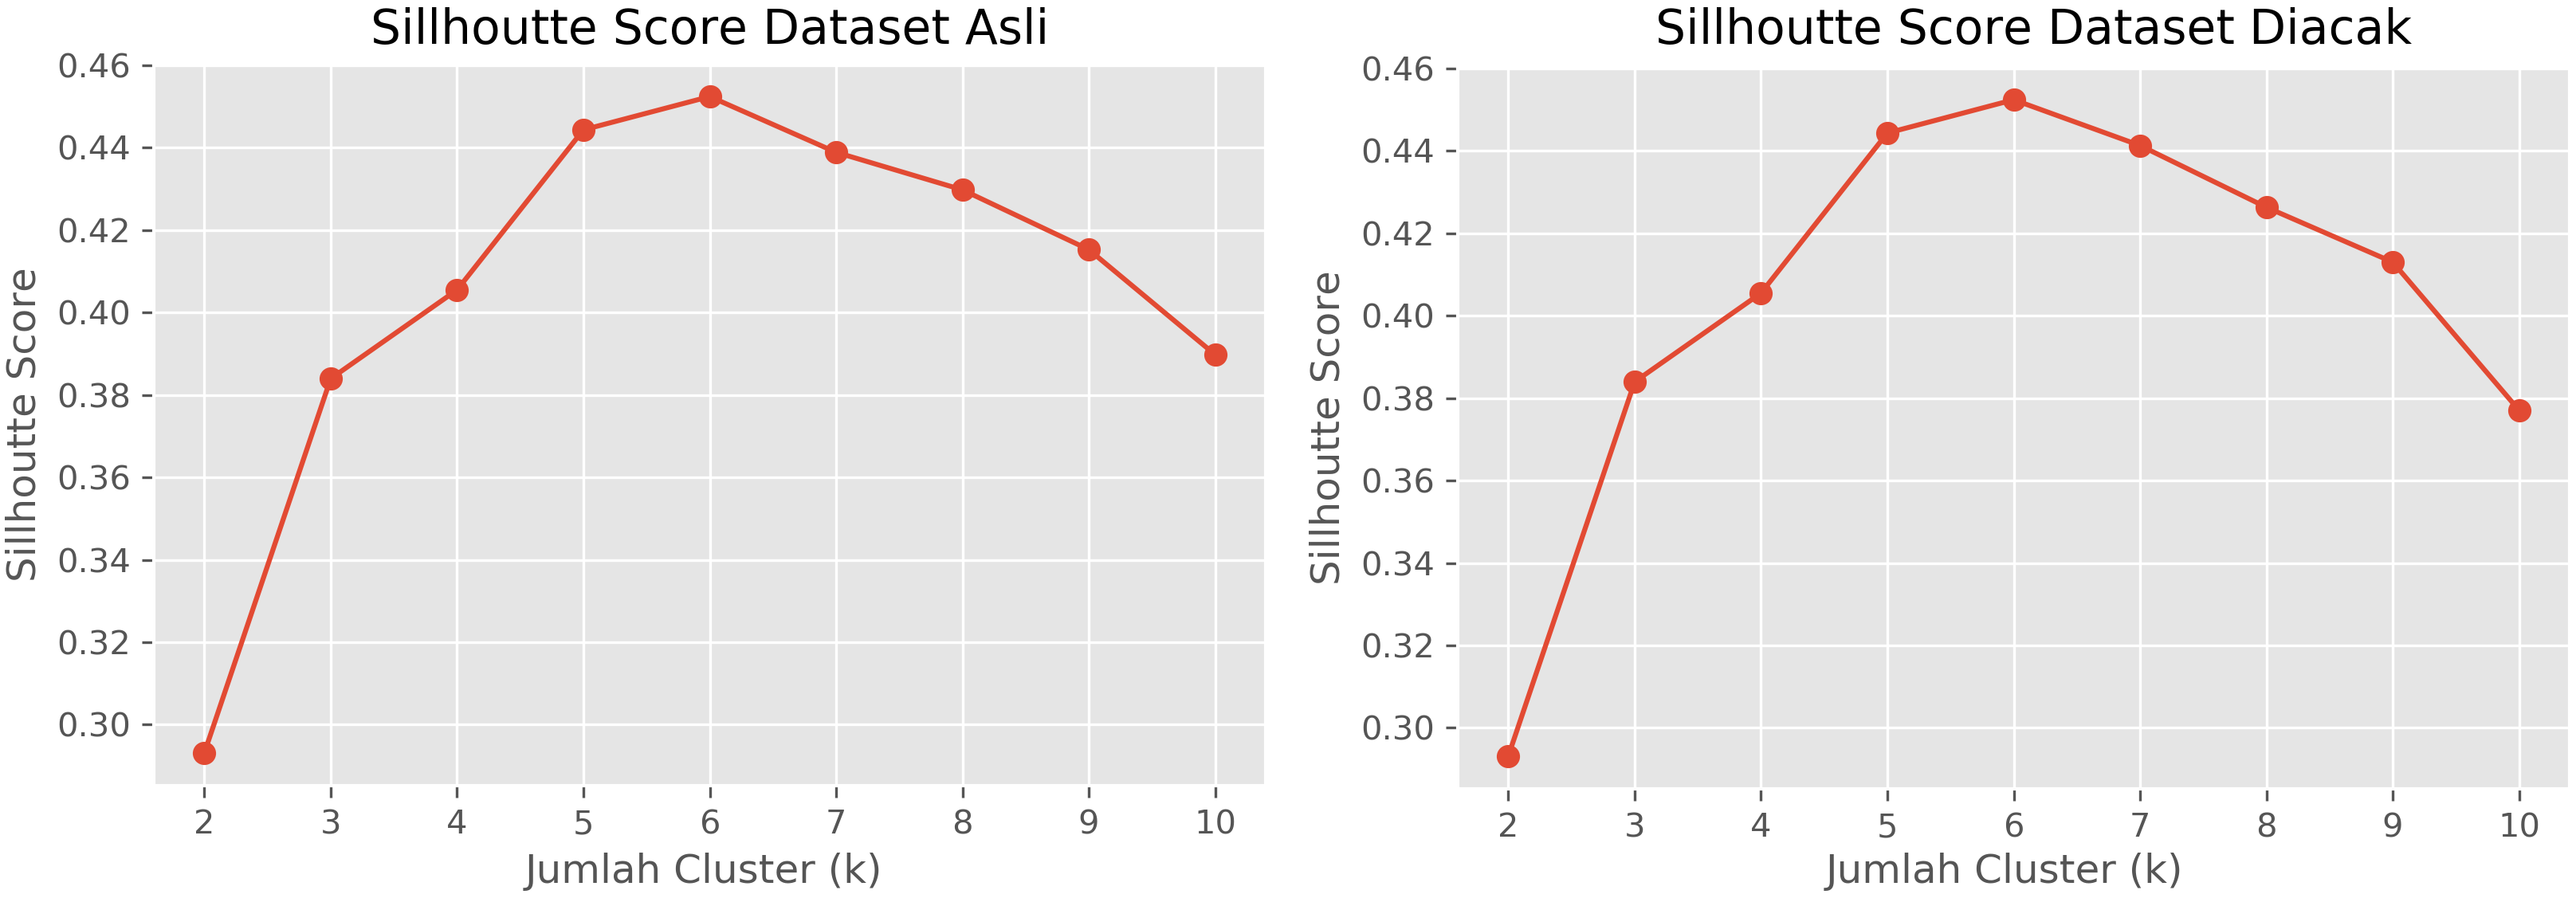
\includegraphics[scale=0.185]{siluet_mall_customers}
	\caption{Grafik \textit{Silhoutte Score} model \textit{clustering} pada \textit{dataset} \textit{mall\_customers}}
	\label{fig:siluet_mall_customers}
\end{figure}
	
\noindent\begin{minipage}{.46\textwidth}
\begin{lstlisting}[caption=\textit{Dataset mall\_customers} Asli,frame=tlrb, label=mall_customers_siluet_asli]{Name}
Silhoutte Score setiap K
pada dataset asli: 
2: 0.293166070535953
3: 0.3839349967742105
4: 0.40546302077733304
5: 0.44504314844253573
6: 0.4523443947724053
7: 0.43978902692261157
8: 0.42790288922594905
9: 0.4137641526186506
10: 0.3750147687842441
\end{lstlisting}
\end{minipage}\hfill
\begin{minipage}{.46\textwidth}
\begin{lstlisting}[caption=\textit{Dataset mall\_customers} Teracak,frame=tlrb, label=mall_customers_siluet_randomisasi]{Name}
Silhoutte Score setiap K
pada dataset teracak: 
2: 0.29316607053507854
3: 0.383934996807901
4: 0.40546302082487856
5: 0.44428597567883826
6: 0.4523443947780976
7: 0.44128075766857394
8: 0.42815090435529995
9: 0.3861502477348431
10: 0.3897532214988177
\end{lstlisting}
\end{minipage}

Teknik penambangan data \textit{k-means} diterapkan menggunakan 4 buah fitur yang ada untuk menguji apakah \textit{dataset} asli dan \textit{dataset} yang telah diacak menghasilkan kluster dan bentuk yang sama dengan sudut yang berbeda saat divisualisasikan. Pengujian tersebut didasarkan pada sifat teknik \textit{Random Rotation Perturbation} yang menjamin jarak Euclidean setiap titik tidak berubah sama sekali tetapi merotasi seluruh titik yang ada pada bidang Euclidean. Visualisasi \textit{cluster} pada \textit{dataset} asli dan \textit{dataset} yang telah diacak masing-masing dapat dilihat pada Gambar~\ref{fig:kmeans_mall_asli} dan Gambar~\ref{fig:kmeans_mall_rotated}. Implementasi kode teknik penambangan data ini diterapkan dengan bahasa pemograman Python dan dibantu oleh \textit{library} Scikit-learn. Visualisasi model \textit{clustering} dengan nilai \textit{k} sebesar 6 pada \textit{dataset} \textit{mall\_customers} asli dan yang telah diacak dapat dilihat pada Gambar~\ref{fig:kmeans_mall_asli} dan Gambar~\ref{fig:kmeans_mall_rotated}. 

\begin{figure}
	\centering
	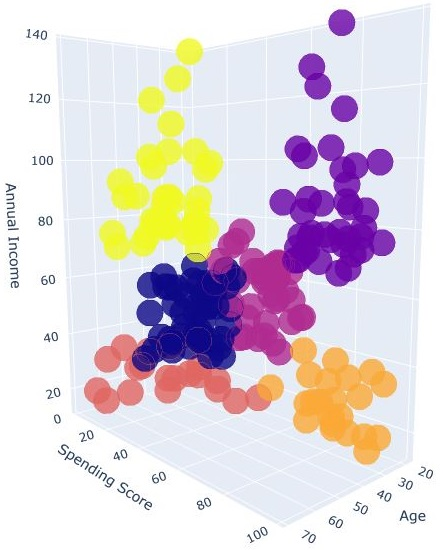
\includegraphics[scale=1]{kmeans_mall_asli}
	\caption{Visualisasi \textit{cluster} pada \textit{dataset} yang asli}
	\label{fig:kmeans_mall_asli}
\end{figure}

\begin{figure}
	\centering
	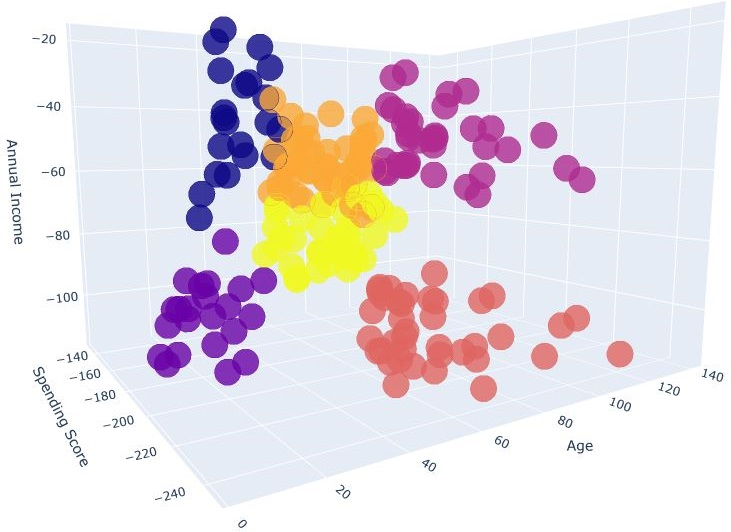
\includegraphics[scale=0.7]{kmeans_mall_rotated}
	\caption{Visualisasi \textit{cluster} pada \textit{dataset} yang telah dirotasi}
	\label{fig:kmeans_mall_rotated}
\end{figure}

Dapat dilihat pada kedua visualisasi tersebut mempunyai jumlah \textit{cluster} yang sama dan terlihat dari lokasi titik-titik yang ada jika dibandingkan terlihat seperti dirotasi searah jarum jam dan bentuknya masih terlihat sama. Apabila dihitung kemiripan \textit{cluster} tersebut dengan metode \textit{Adjusted Rand Index} maka kedua hasil \textit{clustering} tersebut mempunyai nilai 1.0 yang berarti titik-titik yang ada pada setiap \textit{cluster} pada kedua model persis adanya.
	
Waktu eksekusi yang dibutuhkan untuk melatih model \textit{clustering} dengan algoritma \textit{k-means} adalah 0.02995157241821289 detik pada \textit{dataset} yang asli dan 0.032910823822021484 detik pada \textit{dataset} yang telah diacak, hal ini menunjukkan bahwa teknik \textit{Random Rotation Perturbation} tidak memepengaruhi secara signifikan waktu eksekusi untuk melatih model \textit{k-means}.

\subsubsection{\textit{Random Projection Perturbation}}
\label{subsubsec:pengujian-clustering-rpp}

Pengujian teknik \textit{Random Projection Perturbation} untuk penambangan data \textit{clustering} dengan algoritma \textit{k-means} akan dilakukan dengan \textit{dataset} \textit{mobile\_sensor} yang dapat dilihat 20 baris pertamanya pada Gambar~\ref{fig:mobile_sensor_asli}. \textit{Dataset} ini diacak dengan teknik \textit{Random Projection Perturbation} dan hasil pengacakan dapat dilihat pada Gambar~\ref{fig:projected_mobile_sensor}. Dengan kedua \textit{dataset} tersebut, dilakukan penambangan data terhadap kedua \textit{dataset} tersebut dan dihasilkan berbagai macam informasi yang dapat dibandingkan. Berikut adalah hasil pengujian dan penjelasannya.

Sebelum melakukan teknik \textit{clustering} dengan algoritma \textit{k-means}, \textit{dataset} yang memiliki fitur yang sangat banyak tersebut dimensinya harus direduksi terlebih dahulu agar model dapat divisualisasikan dengan mudah. \textit{Dataset} yang akan di-\textit{cluster} akan direduksi dimensinya sampai hanya memiliki 2 dimensi. Reduksi dimensi dilakukan dengan menerapkan teknik \textit{Principal Component Analysis} yang sudah umum digunakan saat penambangan data dan hasilnya relatif baik. Dalam menguji teknik \textit{Random Projection Perturbation}, \textit{dataset} yang tidak diterapkan teknik tersebut langsung direduksi dimensinya dengan teknik \textit{Principal Component Analysis}. \textit{Dataset} yang akan diacak akan terlebih dahulu diterapkan teknik \textit{Random Projection Perturbation} baru direduksi dimensinya menjadi 2 dimensi dengan teknik \textit{Principal Component Analysis}.

Pada Gambar~\ref{fig:elbow_mobile_sensor} terdapat grafik \textit{Sum of Squared Error} untuk menggunakan metode Elbow pada \textit{dataset} asli dan \textit{dataset} yang telah diacak. Pada grafik ini tidak terlalu terlihat nilai yang terbaik untuk menjadi nilai \textit{k} yang dipakai pada \textit{dataset} asli maupun \textit{dataset} yang telah diacak. Walaupun seperti itu, pada kedua \textit{dataset} tersebut grafik \textit{Sum of Squared Error}-nya terlihat sangat mirip dikarenakan teknik \textit{Random Projection Perturbation} menjaga jarak Euclidean dengan baik dan terkontrol. Dalam menentukan nilai \textit{k} yang terbaik untuk dipakai membuat model, \textit{Silhoutte Score} dapat digunakan untuk metode alternatif untuk menentukan nilai \textit{k} yang terbaik.

\begin{figure}
	\centering
	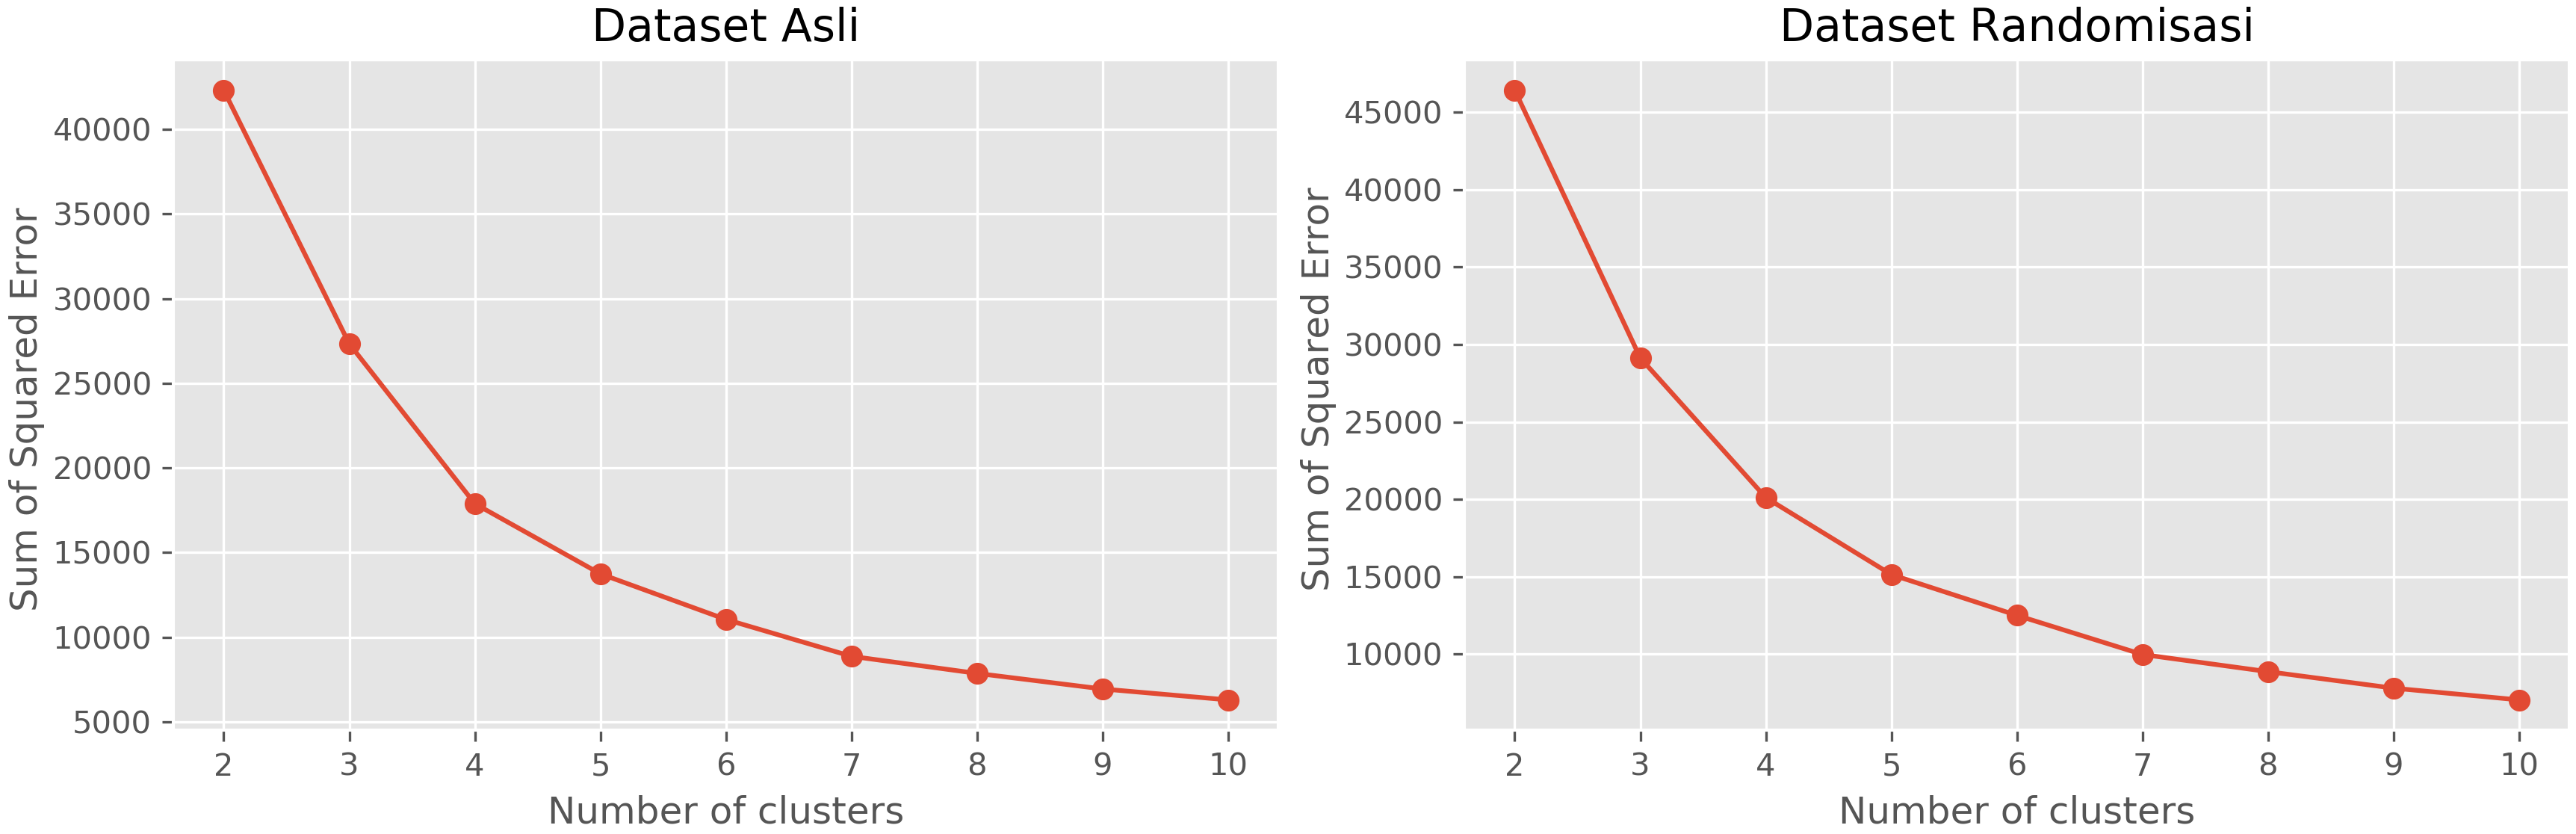
\includegraphics[scale=0.18]{elbow_mobile_sensor}
	\caption{Grafik \textit{Sum of Squared Error} model \textit{clustering} pada \textit{dataset} \textit{mobile\_sensor}}
	\label{fig:elbow_mobile_sensor}
\end{figure}

Pada Gambar~\ref{fig:siluet_mobile_sensor} terdapat grafik \textit{Silhoutte Score} dari \textit{dataset} \textit{mobile\_sensor} yang asli dan yang telah diacak. Dapat terlihat kedua grafik \textit{Silhoutte Score} terlihat sangat mirip dan dapat dilihat nilai-nilai pada setiap \textit{k} tersebut di Listing~\ref{mobile_sensor_siluet_asli} dan Listing~\ref{mobile_sensor_siluet_randomisasi} ada sedikit perbedaan yang tidak terlalu signifikan. Hal ini dikarenakan oleh jarak Euclidean pada \textit{dataset} asli dan yang telah diacak sedikit berbeda sehingga mempengaruhi sedikit pada hasil algoritma \textit{Silhoutte Score}. Dapat terlihat \textit{Silhoutte Score} pada nilai \textit{k} sebesar 2 adalah nilai paling besar yaitu 0.7568010158989575 pada \textit{dataset} asli dan 0.7581796759180272 pada \textit{dataset} yang telah diacak. Hal ini menunjukkan teknik \textit{Random Projection Perturbation} tidak mempengaruhi secara signifikan nilai \textit{Silhoutte Score} pada setiap \textit{k}.

\begin{figure}
	\centering
	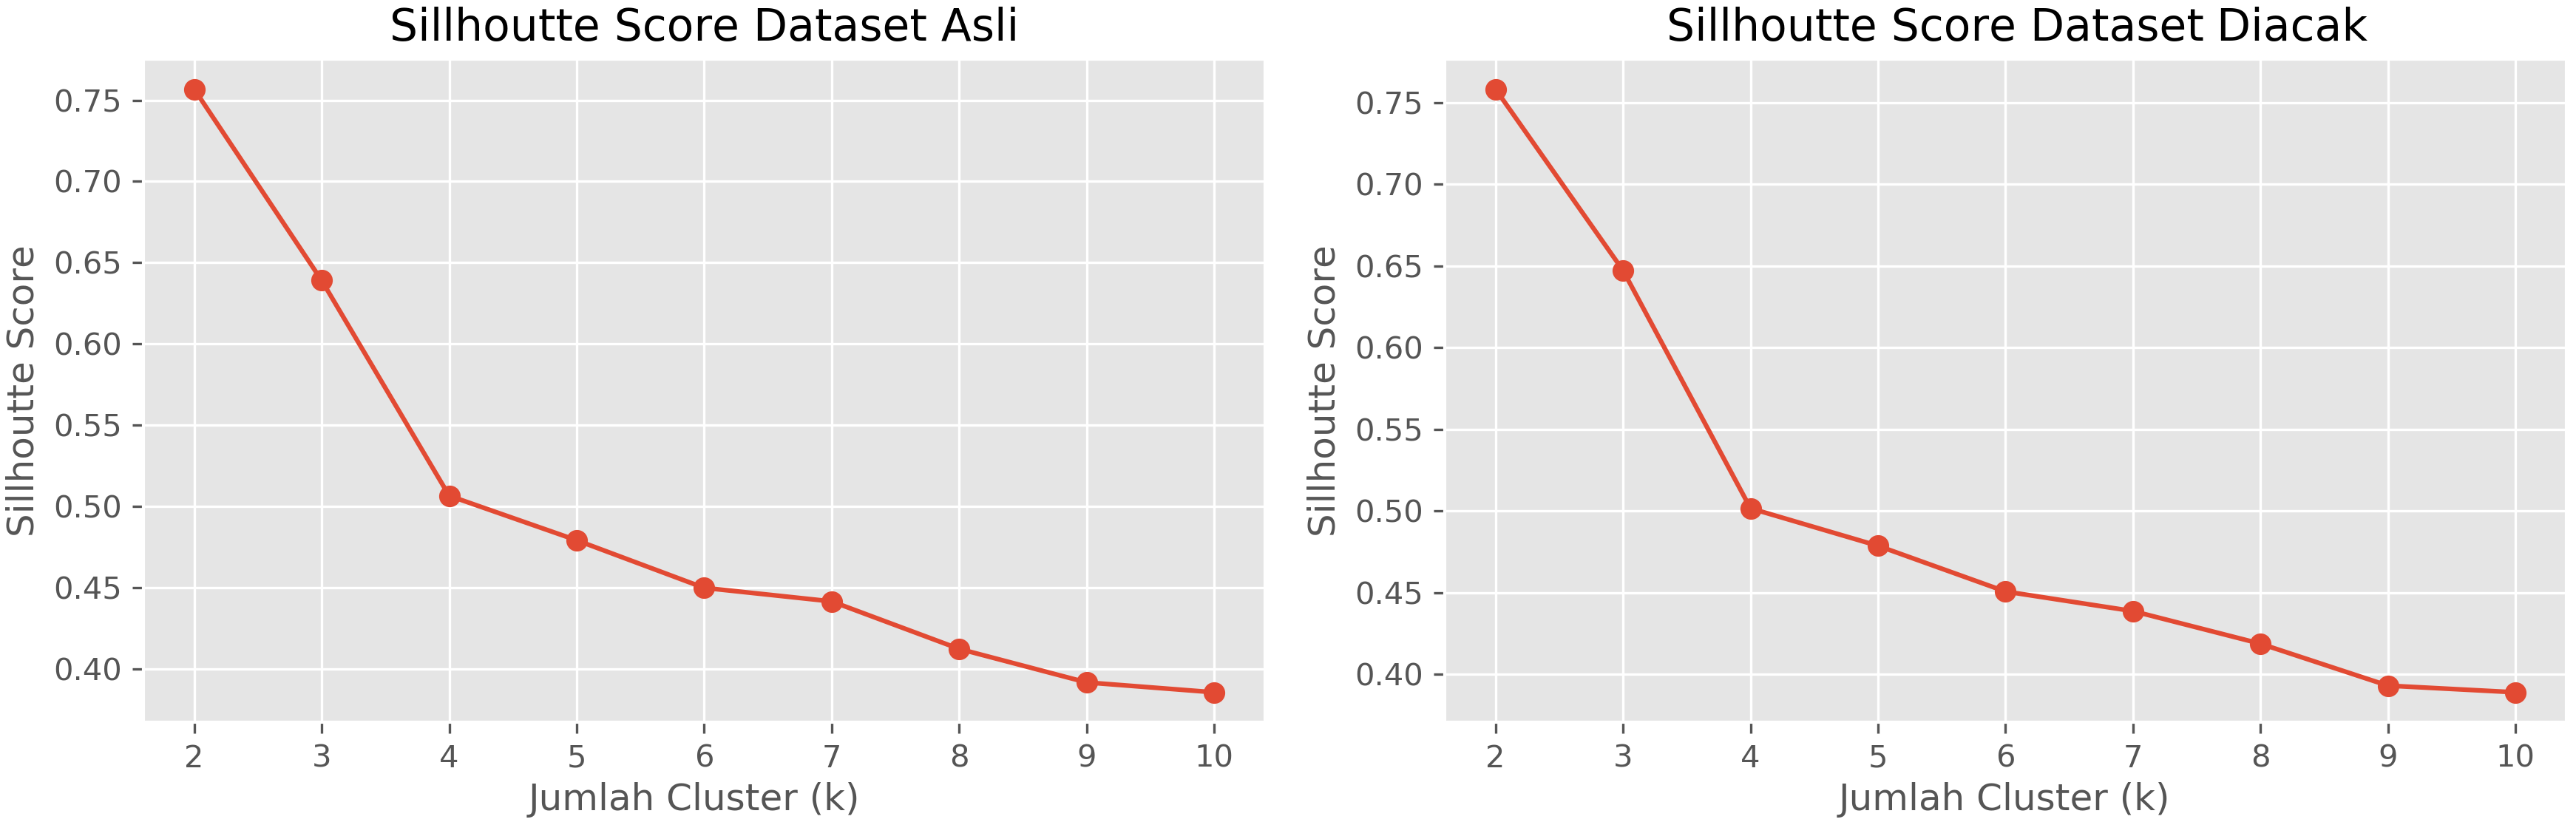
\includegraphics[scale=0.175]{siluet_mobile_sensor}
	\caption{Grafik \textit{Silhoutte Score} model \textit{clustering} pada \textit{dataset} \textit{mobile\_sensor}}
	\label{fig:siluet_mobile_sensor}
\end{figure}
	
\noindent\begin{minipage}{.46\textwidth}
\begin{lstlisting}[caption=\textit{Dataset mobile\_sensor} Asli,frame=tlrb, label=mobile_sensor_siluet_asli]{Name}
Silhoutte Score setiap K
pada dataset asli: 
2: 0.7568010158989575
3: 0.6390101777235029
4: 0.506497255331499
5: 0.4790910470659918
6: 0.4497981866661921
7: 0.4414685328088866
8: 0.4122363491089296
9: 0.39158160384319435
10: 0.3854996654126945
\end{lstlisting}
\end{minipage}\hfill
\begin{minipage}{.46\textwidth}
\begin{lstlisting}[caption=\textit{Dataset mobile\_sensor} Teracak,frame=tlrb, label=mobile_sensor_siluet_randomisasi]{Name}
Silhoutte Score setiap K
pada dataset teracak: 
2: 0.7581796759180272
3: 0.6472419899391577
4: 0.5015650888399312
5: 0.47862510668209096
6: 0.45064475921629954
7: 0.43865532313764366
8: 0.4186927518384631
9: 0.3930205669353965
10: 0.3889412224520463
\end{lstlisting}
\end{minipage}

Teknik penambangan data \textit{k-means} diterapkan menggunakan dua buah fitur yang ada hasil dari teknik \textit{Principal Component Analysis} untuk menguji apakah \textit{dataset} asli dan \textit{dataset} yang telah diacak menghasilkan \textit{cluster} yang hampir sama. Pengujian tersebut didasarkan pada sifat teknik \textit{Random Projection Perturbation} yang menjamin jarak Euclidean terjaga dengan besar distorsi yang ditentukan pengguna. Model \textit{k-means} akan dibuat dengan nilai \textit{k} yang terbaik dihitung menggunakan metode Elbow dan nilai \textit{k} yang memiliki \textit{Silhoutte Score} tertinggi. Implementasi kode teknik penambangan data ini diterapkan dengan bahasa pemograman Python dan dibantu oleh \textit{library} Scikit-learn. 

Visualisasi model \textit{clustering} dengan nilai \textit{k} sebesar 2 pada \textit{dataset} \textit{mobile\_sensor} asli dan yang telah diacak dapat dilihat pada Gambar~\ref{fig:kmeans_mobile_sensor_asli} dan Gambar~\ref{fig:kmeans_mobile_sensor_randomisasi}. Dapat dilihat pada kedua visualisasi tersebut mempunyai jumlah \textit{cluster} yang sama yaitu 2 \textit{cluster} dan terlihat dari lokasi titik-titik yang ada jika dibandingkan ada sedikit perbedaan tetapi tidak terlalu signifikan. Hasil \textit{clustering} menyatakan bahwa ada dua buah \textit{cluster} yaitu kelompok orang-orang yang diam dan kelompok orang-orang yang bergerak, hasil \textit{clustering} ini tidak secara spesifik menentukan aktivitas setiap orang karena informasi tersebut sudah hilang oleh teknik yang digunakan sebelumnya, \textit{Principal Component Analysis}. 
	
\begin{figure}
	\centering
	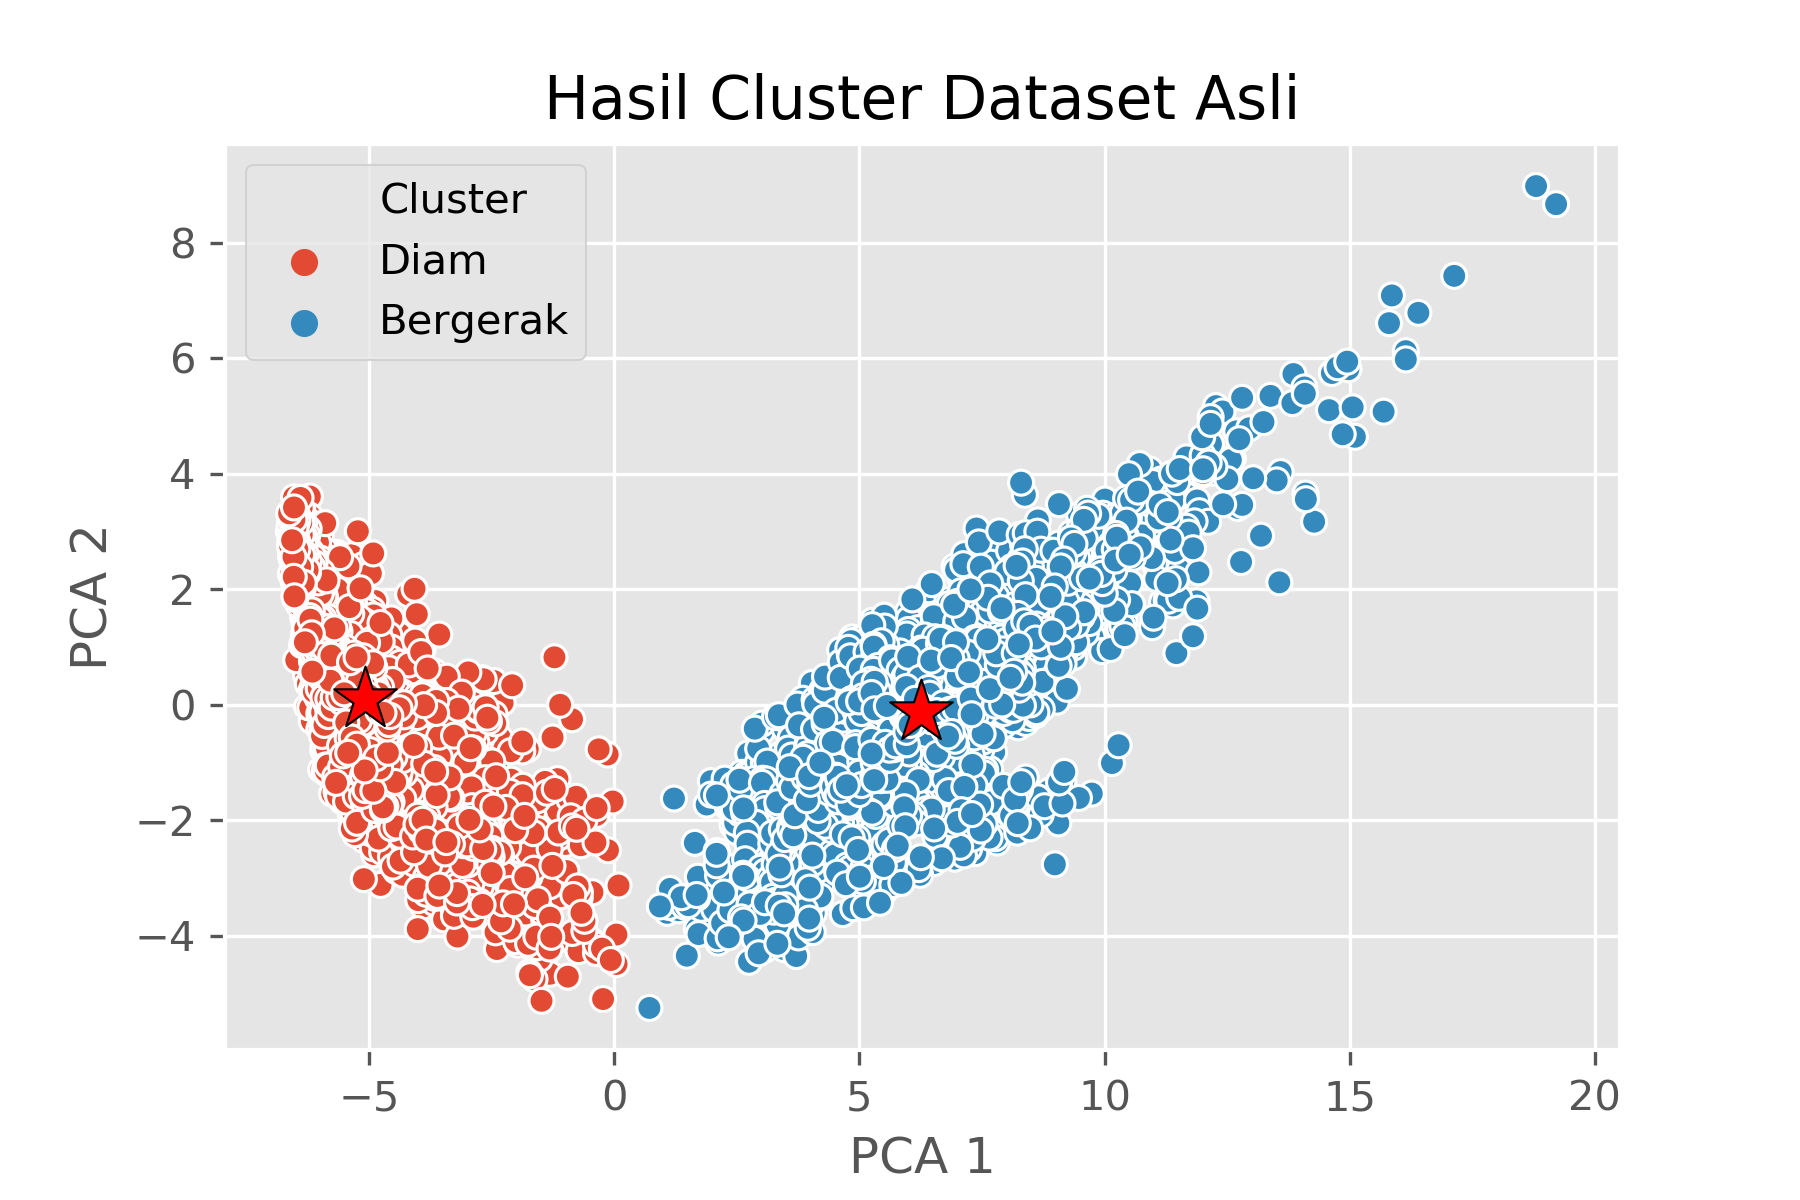
\includegraphics[scale=1]{kmeans_mobile_sensor_asli}
	\caption{Visualisasi \textit{cluster} pada \textit{dataset} yang asli}
	\label{fig:kmeans_mobile_sensor_asli}
\end{figure}

\begin{figure}
	\centering
	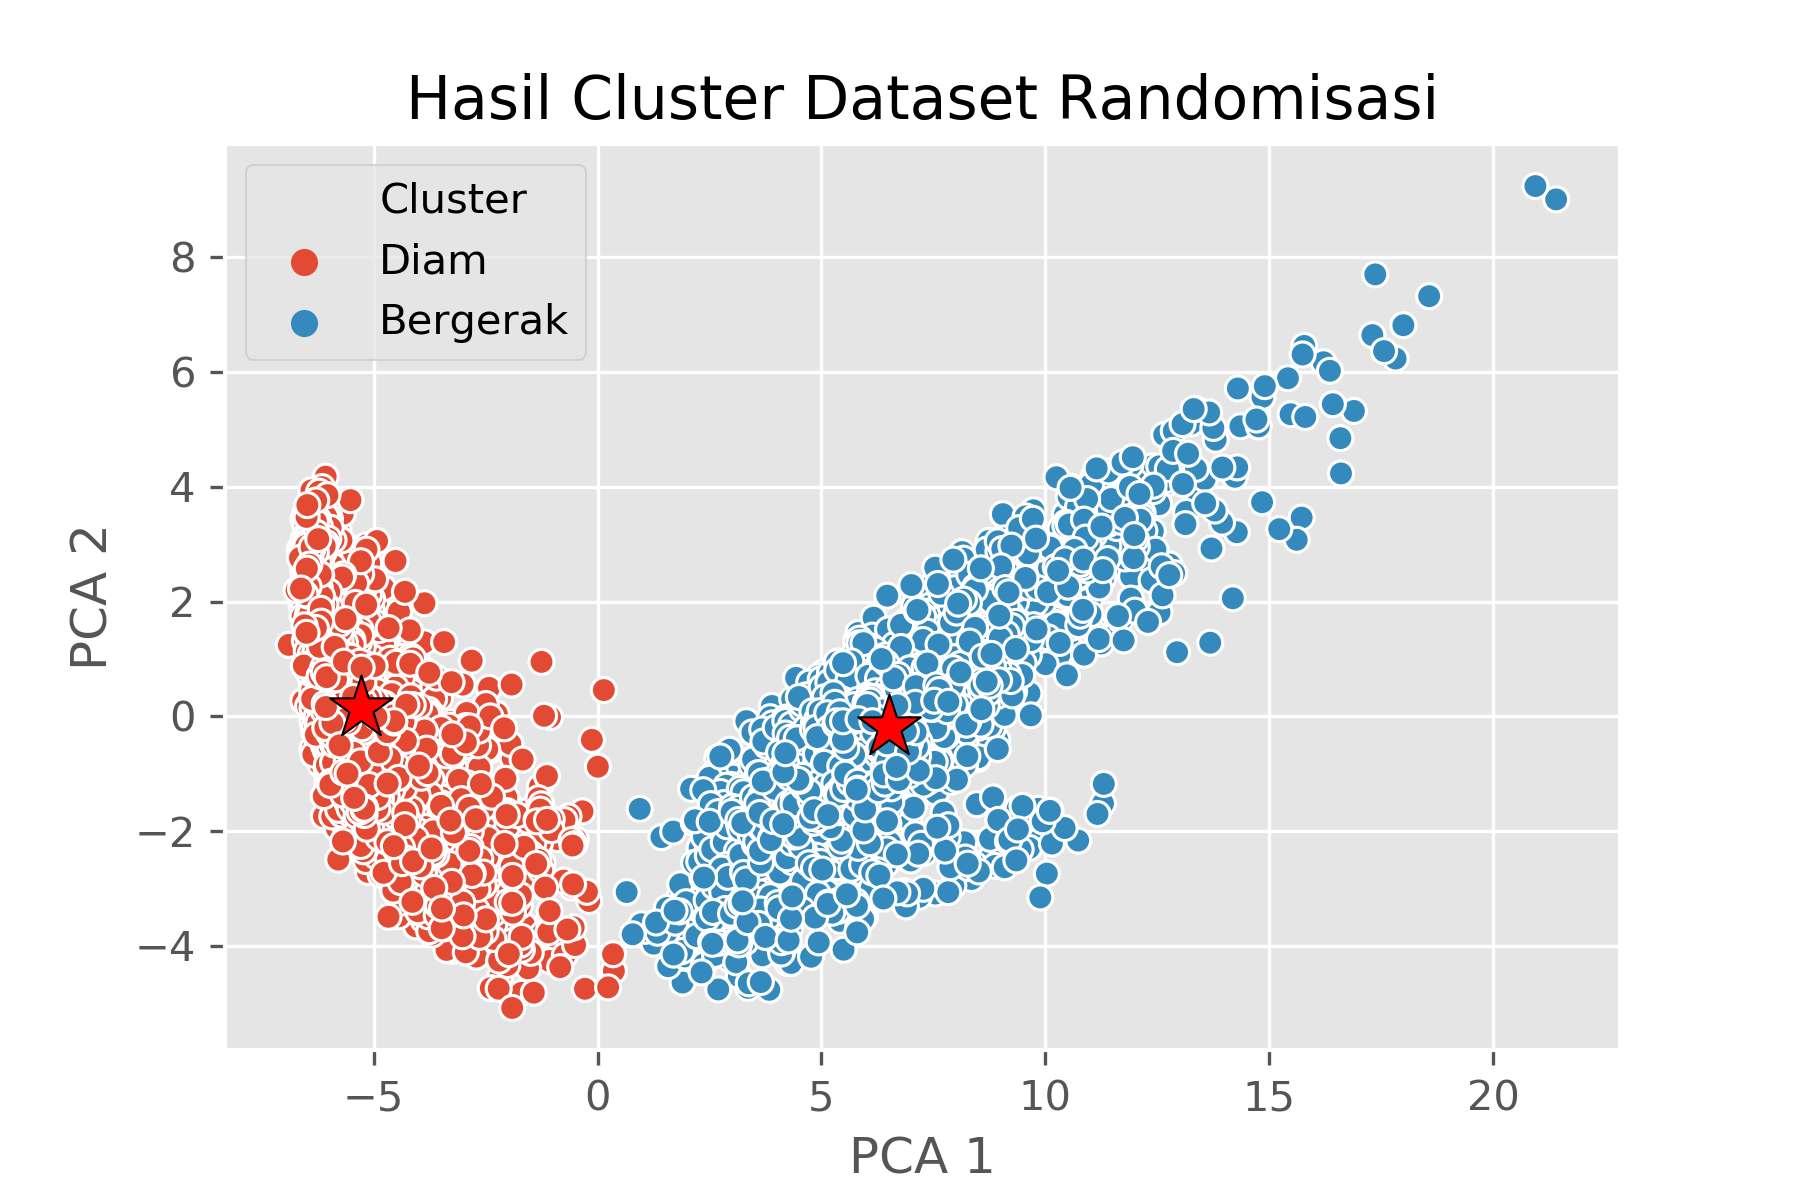
\includegraphics[scale=1]{kmeans_mobile_sensor_randomisasi}
	\caption{Visualisasi \textit{cluster} pada \textit{dataset} yang telah diproyeksi}
	\label{fig:kmeans_mobile_sensor_randomisasi}
\end{figure}
	
Apabila dihitung kemiripan \textit{cluster} tersebut dengan metode \textit{Adjusted Rand Index} maka kedua hasil \textit{clustering} tersebut mempunyai nilai 0.9994558701020273 yang berarti titik-titik yang ada pada setiap \textit{cluster} pada kedua model sangat mirip sekali. Hal ini dikarenakan jarak Euclidean kedua buah \textit{dataset} tidak rusak secara signifikan dan distorsinya terkendali sesuai yang pengguna inginkan.

Waktu eksekusi yang dibutuhkan untuk melatih model \textit{k-means} dengan nilai \textit{k} sebesar 2 adalah sebesar 0.031239032745361328 detik pada \textit{dataset} asli dan 0.031217575073242188 detik pada \textit{dataset} yang telah diacak. Jika dibandingkan, kedua \textit{dataset} memiliki waktu eksekusi yang hampir sama, hal ini dikarenakan kedua \textit{dataset} tersebut diterapkan terlebih dahulu teknik \textit{Principal Component Analysis} sehingga kedua \textit{dataset} memiliki ukuran yang sama. Perbedaan pada kedua \textit{dataset} dapat terlihat pada waktu eksekusi teknik \textit{Principal Component Analysis} pada kedua \textit{dataset} yang mana masing-masing sebesar 0.1405951976776123 detik dan 0.1093449592590332 detik. Oleh karena itu, teknik \textit{Random Projection Perturbation} mempengaruhi waktu eksekusi karena ukuran \textit{dataset} berkurang sehingga waktu eksekusinya juga berkurang.

\subsubsection{Kesimpulan}
\label{subsubsec:pengujian-clustering-kesimpulan}

Berdasarkan pengujian dengan teknik penambangan data \textit{clustering} menggunakan teknik \textit{k-means} pada \textit{dataset} asli, \textit{dataset} yang telah diacak menggunakan teknik \textit{Random Rotation Perturbation}, dan \textit{dataset} yang telah diacak menggunakan teknik \textit{Random Projection Perturbation} dibuat kesimpulan sekaligus membandingkan antara kedua teknik \textit{Randomization}. Pada Tabel~\ref{table:perbandingan-clustering} dapat dilihat hasil akhir pengujian antara model yang dilatih dengan \textit{dataset} asli dan \textit{dataset} yang telah diacak dengan \textit{Random Rotation Perturbation} dan \textit{Random Projection Perturbation}.

\begin{table}
	\centering
	\caption{Perbandingan Model \textit{k-means}}
	\begin{tabular}{|l|l|l|}
		\hline
		& \textbf{\textit{Rotation}} & \textbf{\textit{Projection}} \\ \hline
		\textbf{\textit{Sum of Squared Error}} & Sangat Mirip & Sangat Mirip \\
		\textbf{\textit{Silhoutte Score}} & Sangat Mirip & Sangat Mirip \\
		\textbf{Jumlah \textit{cluster}} & Sama & Sama \\
		\textbf{Visualisasi \textit{cluster}} & Sedikit Berbeda & Sedikit Berbeda \\
		\textbf{Nilai \textit{Adjusted Rand Index}} & 1.0 & Sangat Mendekati 1.0 \\
		\textbf{Waktu Eksekusi} & Sama & Lebih Cepat \\
		\hline
	\end{tabular}
	\label{table:perbandingan-clustering}
\end{table}

Model \textit{clustering} yang dilatih oleh \textit{dataset} yang diacak sangat mirip dengan \textit{dataset} asli. \textit{Sum of Squared Error} dan \textit{Silhoutte Score} pada kedua teknik \textit{Randomization} memiliki hasil yang sangat mirip dengan aslinya sehingga metode Elbow dan pemilihan fitur dengan \textit{Silhoutte Score} dapat dilakukan setelah \textit{dataset} diacak. Jumlah \textit{cluster} (nilai variabel \textit{k}) sama pada kedua teknik dengan sebelum diacak. Visualisasi \textit{cluster} pada kedua teknik sedikit berbeda karena teknik \textit{Random Rotation Perturbation} merotasi seluruh data sehingga visualisasinya akan terotasi dan teknik \textit{Random Projection Perturbation} tidak menjaga jarak Euclidean secara sempurna. \textit{Adjusted Rand Index} pada kedua teknik memiliki nilai yang baik yaitu bernilai 1 atau mendekati 1. Hal ini menunjukkan bahwa model \textit{clustering} antara yang dilatih dengan \textit{dataset} yang telah diacak dan \textit{dataset} aslinya sama persis atau sangat mirip. Waktu eksekusi pembuatan model dan prediksi hanya memiliki perbedaan pada model yang menggunakan \textit{dataset} yang telah diacak dengan teknik \textit{Random Projection Perturbation}. Waktu eksekusinya lebih cepat dikarenakan oleh \textit{dataset} setelah diacak memiliki fitur yang lebih sedikit karena dimensinya direduksi.

\subsection{Kesimpulan Akhir Pengujian Eksperimental}
\label{subsec:kesimpulan-eksperimental}

Berdasarkan hasil pengujian eksperimental dapat disimpulkan bahwa teknik \textit{Random Rotation Perturbation} dan \textit{Random Projection Perturbation} dapat digunakan untuk menghilangkan privasi pada data dengan mengacak data tersebut tetapi masih dapat digunakan untuk penambangan data klasifikasi dan \textit{clustering} masing-masing dengan teknik \textit{k-nearest neighbors} dan \textit{k-means} dengan hasil yang sama dengan \textit{dataset} asli untuk teknik \textit{Random Rotation Perturbation} dan hasil yang sangat mirip dengan \textit{dataset} asli untuk teknik \textit{Random Projection Perturbation}. Hal tersebut dikarenakan teknik \textit{Random Rotation Perturbation} menjaga jarak Euclidean secara sempurna sementara teknik \textit{Random Projection Perturbation} tidak menjaga secara sempurna karena ada distorsi yang terkontrol pada jarak Euclidean setiap titik pada \textit{dataset} yang diacak. 

Ada persyaratan yang harus dipenuhi untuk teknik \textit{Random Projection Perturbation} bekerja dengan baik yaitu data yang dipakai harus cukup besar. Teknik \textit{Random Projection Perturbation} juga memiliki waktu eksekusi untuk melakukan pengacakan dan pembuatan model yang lebih cepat daripada teknik \textit{Random Rotation Perturbation}. Oleh karena itu, teknik \textit{Random Projection Perturbation} lebih cocok dipakai untuk \textit{dataset} yang sangat besar. Sedangkan teknik \textit{Random Rotation Perturbation} masih dapat dipakai untuk \textit{dataset} yang besar juga tetapi tidak mendapatkan keuntungan waktu eksekusi yang lebih cepat seperti teknik \textit{Random Projection Perturbation}. Teknik \textit{Random Rotation Perturbation} lebih cocok digunakan apabila penambangan data klasifikasi atau \textit{clustering} yang dilakukan diharapkan memiliki hasil yang tidak memiliki perbedaan sama sekali dengan penambangan data klasifikasi atau \textit{clustering} yang menggunakan \textit{dataset} asli. 